\documentclass[UTF8,a4paper,zihao=-4,fontset=none]{ctexart}
\newcommand{\ReportHeadLeft}{因子赛道 ｜ 策略研究报告}
\newcommand{\ReportHeadRight}{2026 年 11 月}
% 决赛策略研究报告 公共导言（XeLaTeX + ctexart）
% 原则：层级清楚（章、节两级为主，最多到小节）；正文成段；不用彩色框、侧栏、底纹、小字注释。
% 图表标题在上，写成「图 1　标题（数据范围）」，数据来源写进标题括号或正文，不另起小字行。
%
% 用法：
%   \documentclass[UTF8,a4paper,zihao=-4,fontset=none]{ctexart}
%   % 决赛策略研究报告 公共导言（XeLaTeX + ctexart）
% 原则：层级清楚（章、节两级为主，最多到小节）；正文成段；不用彩色框、侧栏、底纹、小字注释。
% 图表标题在上，写成「图 1　标题（数据范围）」，数据来源写进标题括号或正文，不另起小字行。
%
% 用法：
%   \documentclass[UTF8,a4paper,zihao=-4,fontset=none]{ctexart}
%   % 决赛策略研究报告 公共导言（XeLaTeX + ctexart）
% 原则：层级清楚（章、节两级为主，最多到小节）；正文成段；不用彩色框、侧栏、底纹、小字注释。
% 图表标题在上，写成「图 1　标题（数据范围）」，数据来源写进标题括号或正文，不另起小字行。
%
% 用法：
%   \documentclass[UTF8,a4paper,zihao=-4,fontset=none]{ctexart}
%   \input{../_style/report_preamble.tex}
%   \title{…} \subtitle{…} \team{…} \reportdate{…}
%   \begin{document} \makereporttitle ...

\setCJKmainfont{Songti SC}[BoldFont={Songti SC Bold}]
\def\yhpath{/Applications/Microsoft PowerPoint.app/Contents/Resources/DFonts/}
\setCJKsansfont{msyh.ttc}[Path=\yhpath,BoldFont=msyhbd.ttc]
\setCJKmonofont{msyh.ttc}[Path=\yhpath]
\setmainfont{Times New Roman}
\setsansfont{msyh.ttc}[Path=\yhpath,BoldFont=msyhbd.ttc]
\setmonofont{Menlo}[Scale=0.88]

\usepackage{newunicodechar}
\newunicodechar{→}{\ensuremath{\rightarrow}}
\newunicodechar{≈}{\ensuremath{\approx}}
\newunicodechar{≤}{\ensuremath{\leq}}
\newunicodechar{≥}{\ensuremath{\geq}}
\newunicodechar{−}{\ensuremath{-}}
\newunicodechar{×}{\ensuremath{\times}}
\newunicodechar{÷}{\ensuremath{\div}}
\newunicodechar{±}{\ensuremath{\pm}}
\newunicodechar{β}{\ensuremath{\beta}}
\newunicodechar{λ}{\ensuremath{\lambda}}
\newunicodechar{σ}{\ensuremath{\sigma}}

\usepackage{xcolor}
\definecolor{rnavy}{HTML}{1B365D}
\definecolor{rgrey}{HTML}{7A828C}
\definecolor{rline}{HTML}{BFC5CC}
\definecolor{raccent}{HTML}{C0392B}

\usepackage[a4paper,top=2.6cm,bottom=2.6cm,left=2.7cm,right=2.7cm,headheight=14pt]{geometry}
\linespread{1.45}
\setlength{\parskip}{0.35em}

% 标题层级：章（\section）、节（\subsection）、小节（\subsubsection，少用）
\ctexset{
  section={format=\sffamily\Large\bfseries\color{rnavy}\raggedright, name={,}, number=\arabic{section},
           aftername=\enspace, beforeskip=1.6em, afterskip=0.8em,
           numberformat={\color{white}\colorbox{rnavy}{\makebox[1.1em]{\arabic{section}}}}},
  subsection={format=\sffamily\large\bfseries\color{rnavy}\raggedright, beforeskip=1.2em, afterskip=0.5em},
  subsubsection={format=\sffamily\normalsize\bfseries\raggedright, beforeskip=0.9em, afterskip=0.3em},
}

% 页眉：左栏目、右日期，下方细色线；页脚：页码
\usepackage{fancyhdr}
\providecommand{\ReportHeadLeft}{策略研究报告}
\providecommand{\ReportHeadRight}{2026 年 11 月}
\pagestyle{fancy}
\fancyhf{}
\fancyhead[L]{\sffamily\small\color{rnavy}\ReportHeadLeft}
\fancyhead[R]{\sffamily\small\color{rnavy}\ReportHeadRight}
\renewcommand{\headrule}{{\color{rnavy}\hrule height 0.8pt}}
\fancyfoot[C]{\sffamily\small\thepage}
\fancypagestyle{plain}{\fancyhf{}\renewcommand{\headrulewidth}{0pt}\fancyfoot[C]{\sffamily\small\thepage}}

% 图表：标题在上，「图 1　标题」
\usepackage{graphicx,float}
\usepackage[font=small,labelfont={sf,bf,color=rnavy},textfont={sf,bf,color=rnavy},labelsep=colon,justification=raggedright,singlelinecheck=false,skip=5pt]{caption}
\DeclareCaptionLabelSeparator{zhcolon}{：}
\captionsetup{labelsep=zhcolon}
\captionsetup[figure]{name=图表,position=top}
\captionsetup[table]{name=图表,position=top}
\makeatletter\let\c@table\c@figure\makeatother
% 图表下方一行资料来源（唯一允许的小字）
\newcommand{\source}[1]{\par\vspace{2pt}{\raggedright\sffamily\footnotesize\color{rgrey}资料来源：#1\par}}

\usepackage{booktabs,tabularx,array,multirow}
\renewcommand{\arraystretch}{1.3}
\newcolumntype{L}{>{\raggedright\arraybackslash}X}
\newcolumntype{C}{>{\centering\arraybackslash}X}

\usepackage{amsmath,amssymb,bm}
\usepackage{enumitem}
\setlist{nosep,leftmargin=2em,itemsep=0.2em}

\usepackage{tikz}
\usetikzlibrary{arrows.meta,positioning,calc,fit,decorations.pathreplacing}
\tikzset{
  node/.style = {draw=rnavy, line width=0.6pt, rounded corners=1.5pt, align=flush center,
                 inner xsep=6pt, inner ysep=4pt, font=\sffamily\small},
  key/.style  = {node, draw=raccent, line width=0.8pt},
  soft/.style = {node, draw=rline},
  flow/.style = {-{Stealth[length=2mm]}, line width=0.6pt, draw=rnavy},
  note/.style = {font=\sffamily\small, text=rgrey, align=flush center},
}

% 首页研究要点：每条以一句加粗结论开头
\newenvironment{keypoints}{%
  \par\noindent{\sffamily\large\bfseries\color{rnavy}研究要点}\par\vspace{0.3em}
  {\color{rnavy}\hrule height 0.6pt}\vspace{0.6em}
  \begin{itemize}[leftmargin=1.2em,itemsep=0.6em,label={\color{rnavy}\rule[0.3ex]{0.45em}{0.45em}}]}
  {\end{itemize}\vspace{0.4em}{\color{rline}\hrule height 0.4pt}}
\newcommand{\kp}[1]{{\sffamily\bfseries\color{rnavy}#1}}

\usepackage[hidelinks]{hyperref}
\usepackage{bookmark}

% 封面
\makeatletter
\newcommand{\subtitle}[1]{\gdef\@subtitle{#1}}
\newcommand{\team}[1]{\gdef\@team{#1}}
\newcommand{\reportdate}[1]{\gdef\@reportdate{#1}}
\providecommand{\@subtitle}{}\providecommand{\@team}{}\providecommand{\@reportdate}{}
\newcommand{\makereporttitle}{%
  \thispagestyle{fancy}
  \vspace*{0.4em}
  {\raggedright\sffamily\color{rnavy}\fontsize{20pt}{27pt}\selectfont\bfseries\@title\par}
  \vspace{0.5em}
  {\raggedright\sffamily\large\color{rnavy}\@subtitle\par}
  \vspace{0.3em}
  {\raggedright\sffamily\small\color{rgrey}\@team\qquad\@reportdate\par}
  \vspace{1.2em}}
\makeatother

%   \title{…} \subtitle{…} \team{…} \reportdate{…}
%   \begin{document} \makereporttitle ...

\setCJKmainfont{Songti SC}[BoldFont={Songti SC Bold}]
\def\yhpath{/Applications/Microsoft PowerPoint.app/Contents/Resources/DFonts/}
\setCJKsansfont{msyh.ttc}[Path=\yhpath,BoldFont=msyhbd.ttc]
\setCJKmonofont{msyh.ttc}[Path=\yhpath]
\setmainfont{Times New Roman}
\setsansfont{msyh.ttc}[Path=\yhpath,BoldFont=msyhbd.ttc]
\setmonofont{Menlo}[Scale=0.88]

\usepackage{newunicodechar}
\newunicodechar{→}{\ensuremath{\rightarrow}}
\newunicodechar{≈}{\ensuremath{\approx}}
\newunicodechar{≤}{\ensuremath{\leq}}
\newunicodechar{≥}{\ensuremath{\geq}}
\newunicodechar{−}{\ensuremath{-}}
\newunicodechar{×}{\ensuremath{\times}}
\newunicodechar{÷}{\ensuremath{\div}}
\newunicodechar{±}{\ensuremath{\pm}}
\newunicodechar{β}{\ensuremath{\beta}}
\newunicodechar{λ}{\ensuremath{\lambda}}
\newunicodechar{σ}{\ensuremath{\sigma}}

\usepackage{xcolor}
\definecolor{rnavy}{HTML}{1B365D}
\definecolor{rgrey}{HTML}{7A828C}
\definecolor{rline}{HTML}{BFC5CC}
\definecolor{raccent}{HTML}{C0392B}

\usepackage[a4paper,top=2.6cm,bottom=2.6cm,left=2.7cm,right=2.7cm,headheight=14pt]{geometry}
\linespread{1.45}
\setlength{\parskip}{0.35em}

% 标题层级：章（\section）、节（\subsection）、小节（\subsubsection，少用）
\ctexset{
  section={format=\sffamily\Large\bfseries\color{rnavy}\raggedright, name={,}, number=\arabic{section},
           aftername=\enspace, beforeskip=1.6em, afterskip=0.8em,
           numberformat={\color{white}\colorbox{rnavy}{\makebox[1.1em]{\arabic{section}}}}},
  subsection={format=\sffamily\large\bfseries\color{rnavy}\raggedright, beforeskip=1.2em, afterskip=0.5em},
  subsubsection={format=\sffamily\normalsize\bfseries\raggedright, beforeskip=0.9em, afterskip=0.3em},
}

% 页眉：左栏目、右日期，下方细色线；页脚：页码
\usepackage{fancyhdr}
\providecommand{\ReportHeadLeft}{策略研究报告}
\providecommand{\ReportHeadRight}{2026 年 11 月}
\pagestyle{fancy}
\fancyhf{}
\fancyhead[L]{\sffamily\small\color{rnavy}\ReportHeadLeft}
\fancyhead[R]{\sffamily\small\color{rnavy}\ReportHeadRight}
\renewcommand{\headrule}{{\color{rnavy}\hrule height 0.8pt}}
\fancyfoot[C]{\sffamily\small\thepage}
\fancypagestyle{plain}{\fancyhf{}\renewcommand{\headrulewidth}{0pt}\fancyfoot[C]{\sffamily\small\thepage}}

% 图表：标题在上，「图 1　标题」
\usepackage{graphicx,float}
\usepackage[font=small,labelfont={sf,bf,color=rnavy},textfont={sf,bf,color=rnavy},labelsep=colon,justification=raggedright,singlelinecheck=false,skip=5pt]{caption}
\DeclareCaptionLabelSeparator{zhcolon}{：}
\captionsetup{labelsep=zhcolon}
\captionsetup[figure]{name=图表,position=top}
\captionsetup[table]{name=图表,position=top}
\makeatletter\let\c@table\c@figure\makeatother
% 图表下方一行资料来源（唯一允许的小字）
\newcommand{\source}[1]{\par\vspace{2pt}{\raggedright\sffamily\footnotesize\color{rgrey}资料来源：#1\par}}

\usepackage{booktabs,tabularx,array,multirow}
\renewcommand{\arraystretch}{1.3}
\newcolumntype{L}{>{\raggedright\arraybackslash}X}
\newcolumntype{C}{>{\centering\arraybackslash}X}

\usepackage{amsmath,amssymb,bm}
\usepackage{enumitem}
\setlist{nosep,leftmargin=2em,itemsep=0.2em}

\usepackage{tikz}
\usetikzlibrary{arrows.meta,positioning,calc,fit,decorations.pathreplacing}
\tikzset{
  node/.style = {draw=rnavy, line width=0.6pt, rounded corners=1.5pt, align=flush center,
                 inner xsep=6pt, inner ysep=4pt, font=\sffamily\small},
  key/.style  = {node, draw=raccent, line width=0.8pt},
  soft/.style = {node, draw=rline},
  flow/.style = {-{Stealth[length=2mm]}, line width=0.6pt, draw=rnavy},
  note/.style = {font=\sffamily\small, text=rgrey, align=flush center},
}

% 首页研究要点：每条以一句加粗结论开头
\newenvironment{keypoints}{%
  \par\noindent{\sffamily\large\bfseries\color{rnavy}研究要点}\par\vspace{0.3em}
  {\color{rnavy}\hrule height 0.6pt}\vspace{0.6em}
  \begin{itemize}[leftmargin=1.2em,itemsep=0.6em,label={\color{rnavy}\rule[0.3ex]{0.45em}{0.45em}}]}
  {\end{itemize}\vspace{0.4em}{\color{rline}\hrule height 0.4pt}}
\newcommand{\kp}[1]{{\sffamily\bfseries\color{rnavy}#1}}

\usepackage[hidelinks]{hyperref}
\usepackage{bookmark}

% 封面
\makeatletter
\newcommand{\subtitle}[1]{\gdef\@subtitle{#1}}
\newcommand{\team}[1]{\gdef\@team{#1}}
\newcommand{\reportdate}[1]{\gdef\@reportdate{#1}}
\providecommand{\@subtitle}{}\providecommand{\@team}{}\providecommand{\@reportdate}{}
\newcommand{\makereporttitle}{%
  \thispagestyle{fancy}
  \vspace*{0.4em}
  {\raggedright\sffamily\color{rnavy}\fontsize{20pt}{27pt}\selectfont\bfseries\@title\par}
  \vspace{0.5em}
  {\raggedright\sffamily\large\color{rnavy}\@subtitle\par}
  \vspace{0.3em}
  {\raggedright\sffamily\small\color{rgrey}\@team\qquad\@reportdate\par}
  \vspace{1.2em}}
\makeatother

%   \title{…} \subtitle{…} \team{…} \reportdate{…}
%   \begin{document} \makereporttitle ...

\setCJKmainfont{Songti SC}[BoldFont={Songti SC Bold}]
\def\yhpath{/Applications/Microsoft PowerPoint.app/Contents/Resources/DFonts/}
\setCJKsansfont{msyh.ttc}[Path=\yhpath,BoldFont=msyhbd.ttc]
\setCJKmonofont{msyh.ttc}[Path=\yhpath]
\setmainfont{Times New Roman}
\setsansfont{msyh.ttc}[Path=\yhpath,BoldFont=msyhbd.ttc]
\setmonofont{Menlo}[Scale=0.88]

\usepackage{newunicodechar}
\newunicodechar{→}{\ensuremath{\rightarrow}}
\newunicodechar{≈}{\ensuremath{\approx}}
\newunicodechar{≤}{\ensuremath{\leq}}
\newunicodechar{≥}{\ensuremath{\geq}}
\newunicodechar{−}{\ensuremath{-}}
\newunicodechar{×}{\ensuremath{\times}}
\newunicodechar{÷}{\ensuremath{\div}}
\newunicodechar{±}{\ensuremath{\pm}}
\newunicodechar{β}{\ensuremath{\beta}}
\newunicodechar{λ}{\ensuremath{\lambda}}
\newunicodechar{σ}{\ensuremath{\sigma}}

\usepackage{xcolor}
\definecolor{rnavy}{HTML}{1B365D}
\definecolor{rgrey}{HTML}{7A828C}
\definecolor{rline}{HTML}{BFC5CC}
\definecolor{raccent}{HTML}{C0392B}

\usepackage[a4paper,top=2.6cm,bottom=2.6cm,left=2.7cm,right=2.7cm,headheight=14pt]{geometry}
\linespread{1.45}
\setlength{\parskip}{0.35em}

% 标题层级：章（\section）、节（\subsection）、小节（\subsubsection，少用）
\ctexset{
  section={format=\sffamily\Large\bfseries\color{rnavy}\raggedright, name={,}, number=\arabic{section},
           aftername=\enspace, beforeskip=1.6em, afterskip=0.8em,
           numberformat={\color{white}\colorbox{rnavy}{\makebox[1.1em]{\arabic{section}}}}},
  subsection={format=\sffamily\large\bfseries\color{rnavy}\raggedright, beforeskip=1.2em, afterskip=0.5em},
  subsubsection={format=\sffamily\normalsize\bfseries\raggedright, beforeskip=0.9em, afterskip=0.3em},
}

% 页眉：左栏目、右日期，下方细色线；页脚：页码
\usepackage{fancyhdr}
\providecommand{\ReportHeadLeft}{策略研究报告}
\providecommand{\ReportHeadRight}{2026 年 11 月}
\pagestyle{fancy}
\fancyhf{}
\fancyhead[L]{\sffamily\small\color{rnavy}\ReportHeadLeft}
\fancyhead[R]{\sffamily\small\color{rnavy}\ReportHeadRight}
\renewcommand{\headrule}{{\color{rnavy}\hrule height 0.8pt}}
\fancyfoot[C]{\sffamily\small\thepage}
\fancypagestyle{plain}{\fancyhf{}\renewcommand{\headrulewidth}{0pt}\fancyfoot[C]{\sffamily\small\thepage}}

% 图表：标题在上，「图 1　标题」
\usepackage{graphicx,float}
\usepackage[font=small,labelfont={sf,bf,color=rnavy},textfont={sf,bf,color=rnavy},labelsep=colon,justification=raggedright,singlelinecheck=false,skip=5pt]{caption}
\DeclareCaptionLabelSeparator{zhcolon}{：}
\captionsetup{labelsep=zhcolon}
\captionsetup[figure]{name=图表,position=top}
\captionsetup[table]{name=图表,position=top}
\makeatletter\let\c@table\c@figure\makeatother
% 图表下方一行资料来源（唯一允许的小字）
\newcommand{\source}[1]{\par\vspace{2pt}{\raggedright\sffamily\footnotesize\color{rgrey}资料来源：#1\par}}

\usepackage{booktabs,tabularx,array,multirow}
\renewcommand{\arraystretch}{1.3}
\newcolumntype{L}{>{\raggedright\arraybackslash}X}
\newcolumntype{C}{>{\centering\arraybackslash}X}

\usepackage{amsmath,amssymb,bm}
\usepackage{enumitem}
\setlist{nosep,leftmargin=2em,itemsep=0.2em}

\usepackage{tikz}
\usetikzlibrary{arrows.meta,positioning,calc,fit,decorations.pathreplacing}
\tikzset{
  node/.style = {draw=rnavy, line width=0.6pt, rounded corners=1.5pt, align=flush center,
                 inner xsep=6pt, inner ysep=4pt, font=\sffamily\small},
  key/.style  = {node, draw=raccent, line width=0.8pt},
  soft/.style = {node, draw=rline},
  flow/.style = {-{Stealth[length=2mm]}, line width=0.6pt, draw=rnavy},
  note/.style = {font=\sffamily\small, text=rgrey, align=flush center},
}

% 首页研究要点：每条以一句加粗结论开头
\newenvironment{keypoints}{%
  \par\noindent{\sffamily\large\bfseries\color{rnavy}研究要点}\par\vspace{0.3em}
  {\color{rnavy}\hrule height 0.6pt}\vspace{0.6em}
  \begin{itemize}[leftmargin=1.2em,itemsep=0.6em,label={\color{rnavy}\rule[0.3ex]{0.45em}{0.45em}}]}
  {\end{itemize}\vspace{0.4em}{\color{rline}\hrule height 0.4pt}}
\newcommand{\kp}[1]{{\sffamily\bfseries\color{rnavy}#1}}

\usepackage[hidelinks]{hyperref}
\usepackage{bookmark}

% 封面
\makeatletter
\newcommand{\subtitle}[1]{\gdef\@subtitle{#1}}
\newcommand{\team}[1]{\gdef\@team{#1}}
\newcommand{\reportdate}[1]{\gdef\@reportdate{#1}}
\providecommand{\@subtitle}{}\providecommand{\@team}{}\providecommand{\@reportdate}{}
\newcommand{\makereporttitle}{%
  \thispagestyle{fancy}
  \vspace*{0.4em}
  {\raggedright\sffamily\color{rnavy}\fontsize{20pt}{27pt}\selectfont\bfseries\@title\par}
  \vspace{0.5em}
  {\raggedright\sffamily\large\color{rnavy}\@subtitle\par}
  \vspace{0.3em}
  {\raggedright\sffamily\small\color{rgrey}\@team\qquad\@reportdate\par}
  \vspace{1.2em}}
\makeatother

\title{分钟级截面因子：\\从交易行为到低换手信号}
\subtitle{因子赛道决赛 · 策略研究报告}
\team{fx\hbox{战队}}
\reportdate{2026 年 11 月}

% 浮动体参数：让图表与正文交替排布，减少整页浮动
\renewcommand{\topfraction}{0.88}
\renewcommand{\bottomfraction}{0.6}
\renewcommand{\textfraction}{0.1}
\renewcommand{\floatpagefraction}{0.8}
\setcounter{topnumber}{3}
\setcounter{bottomnumber}{2}
\setcounter{totalnumber}{4}
% 只含浮动体的页面从页首排起，不垂直居中
\makeatletter\setlength{\@fptop}{0pt}\setlength{\@fpbot}{0pt plus 1fil}\makeatother

% 表格内部行距略收紧，只作用于本文件的表格
\newcommand{\tablesetup}{\small\linespread{1.08}\selectfont\renewcommand{\arraystretch}{1.22}}
\newcolumntype{P}[1]{>{\raggedright\arraybackslash}p{#1}}
\usepackage{xltabular}
\newcommand{\figwidth}{\textwidth}

\begin{document}
\makereporttitle

\begin{keypoints}
\item \kp{最终因子在公榜与私榜总榜均列第二，私榜 RankIC 0.0790、ICIR 1.559、换手率 0.266。}因子由三部分组成：16 个浅层梯度提升树组合 27 个基础信号；15 项增量信号补充委托结构、订单流与收盘竞价信息；换手缓冲带在剔除风格与行业之后的排名上控制换手。公榜五项为 RankIC 0.1028、ICIR 2.069、多空组合夏普比率 54.18、压力稳定性 1.953、换手率 0.279。
\item \kp{短期超涨超跌之后的回补是首要信号来源，挂单结构与收盘竞价提供基础组合之外的新信息。}基础组合的分裂权重中，同伴残差反转类占 28.5\%。约 200 个候选逐个加入后，只有委托结构类能使四项质量指标上升且换手率不升：同样的买一挂单量，委托笔数多的随后偏强，单笔规模大的随后偏弱。14:30 截面的标签包含收盘集合竞价，加入只在该截面起作用的增量信号后，其 RankIC 由 0.105 升至 0.128～0.130。
\item \kp{浅层树刻画基础信号的非线性，新信息以小权重逐项线性叠加。}基础组合只在 2020–2022 年拟合，在样本外的 2023、2024 年，RankIC 比同输入的线性合成分别高 0.0095 和 0.0086，非线性集中在反转信号上。新信息作为树的输入时，在相同换手率下五项均不如线性叠加。
\item \kp{换手缓冲带放在剔除风格与行业之后，换手率下降 44\%，RankIC 同步提高。}平台按剔除风格与行业后的排名划分多空组合，缓冲带改用同一口径的排名后，换手率同为 0.357 时 RankIC 由 0.0899 升至 0.0921。从基础组合到最终因子，换手率由 0.518 降至 0.290，RankIC 提高 0.0038，ICIR 提高 0.144，多空组合夏普比率下降 2.59。
\item \kp{同一套增量信号与后处理在未参与筛选的 2020–2022 年同样有效。}以线性合成基准为基础组合，2020–2024 年每年 RankIC 提高 0.0078～0.0086、ICIR 提高 0.196～0.234。私榜 RankIC 较公榜回落 23.2\%，逐截面 RankIC 的标准差由 0.0497 变为 0.0507，换手率由 0.279 降至 0.266。
\item \kp{风险提示：}私榜区间日期未公布，四项质量指标较公榜回落 16\%～28\%，无法与过拟合完全区分；14:30 的效应依赖收盘集合竞价制度；委托结构类信号的单独 RankIC 在 2020–2024 年约减半；未做含交易成本的回测，多空组合夏普比率不代表可实现收益。
\end{keypoints}

{\linespread{1.2}\selectfont\tableofcontents}
\newpage

% ==================================================================
\section{评测口径决定预测目标}\label{sec:ch1}

比赛要求在每个交易日的 8 个截面上对全部股票给出因子值，平台按五项指标在参评提交中的百分位计分。寻找信号之前，我们先在平台上逐项核实了三条口径：标签是截面之后 30 分钟窗口的收盘价相对同窗口成交量加权均价的偏离；五项指标都在对 10 个风格因子与 32 个行业回归取残差之后的排名上计算；换手只统计同一交易日相邻截面之间多空组合的成分变化。这三条口径决定了信号的寻找方向，以及换手控制在计算流程中的位置。我们据此搭建了与平台同口径的本地评测系统，本报告中标注“本地”的数字均出自这套系统。

\subsection{标签衡量半小时窗口内的价格漂移}\label{sec:label}

比赛初期平台没有公布标签定义，按公榜得分反推的口径与官方标签的截面秩相关只有 0.56。团队成员随后在平台上导出 2024 年一季度与 2021 年 6 月两段官方标签表，我们逐行比对后确认了标签的定义，两段数据全部吻合，误差小于 $10^{-7}$：
\begin{equation}
y_{i,t}=\frac{P^{\mathrm{close}}_{i,(t,\,t+30]}}{\mathrm{VWAP}_{i,(t,\,t+30]}}-1,
\end{equation}
其中 $P^{\mathrm{close}}_{i,(t,t+30]}$ 是股票 $i$ 在截面 $t$ 之后 30 分钟窗口的末价，$\mathrm{VWAP}_{i,(t,t+30]}$ 是同一窗口的成交量加权均价。标签的含义是在窗口内按均价买入、在窗口末按收盘价卖出的收益。它与 30 分钟收益率不同：窗口内先跌后涨、收在均价之上的股票，标签为正；30 分钟收益为正但冲高回落的股票，标签可能为负。因此，能预测窗口内价格漂移方向的信号都可以使用，个股在某个半小时内收在均价之上还是之下的习惯本身也可以作为预测依据。

图表~\ref{fig:timeline} 给出每日 8 个截面与对应的标签窗口。窗口首尾相接，覆盖整个连续交易时段，其中两个截面需要单独说明。11:30 截面的窗口跨过午休，对应 13:01–13:30。14:30 截面的窗口末价是 15:00 的收盘集合竞价价，这一标签可以拆成连续竞价漂移（14:57 收盘价相对 14:31–14:57 均价）与收盘竞价跳动（15:00 价格相对 14:57 价格）两部分，两者与标签的截面秩相关分别为 0.73 和 0.38，竞价成交占窗口成交比例的中位数约为 8\%。因此 14:30 截面的标签结构与其他截面不同，第~\ref{sec:1430}~节专门讨论。

\begin{figure}[htbp]
\caption{每日 8 个截面与对应的 30 分钟标签窗口（示意，午休间隔不按比例）}\label{fig:timeline}
\centering
\begin{tikzpicture}[x=1.36cm,y=1cm]
  \draw[rnavy,line width=1.1pt] (0,0) -- (4,0);
  \draw[rnavy,line width=1.1pt] (5.0,0) -- (9.0,0);
  \draw[rnavy,line width=0.6pt] (4.32,-0.13) -- (4.42,0.13);
  \draw[rnavy,line width=0.6pt] (4.58,-0.13) -- (4.68,0.13);
  \foreach \x/\t in {0/09:30,1/10:00,2/10:30,3/11:00,4/11:30,5.0/13:00,6.0/13:30,7.0/14:00,8.0/14:30,9.0/15:00}
    \node[note,below] at (\x,-0.1) {\t};
  \foreach \a/\b in {1/2,2/3,3/4,5.0/6.0,6.0/7.0,7.0/8.0}
    \draw[rnavy,line width=0.9pt,{Bar[width=6pt]}-{Bar[width=6pt]}] (\a+0.04,0.5) -- (\b-0.04,0.5);
  \draw[rline,line width=0.9pt,{Bar[width=6pt]}-{Bar[width=6pt]}] (0.04,0.5) -- (0.96,0.5);
  \draw[raccent,line width=1.1pt,{Bar[width=6pt]}-{Bar[width=6pt]}] (8.04,0.5) -- (8.96,0.5);
  \foreach \x in {1,2,3,4,6.0,7.0}
    \fill[rnavy] (\x,0) circle (2.3pt);
  \fill[rline] (0,0) circle (2.3pt);
  \fill[raccent] (8.0,0) circle (2.8pt);
  \draw[flow,draw=rgrey] (4.02,0.12) .. controls (4.2,1.15) and (5.1,1.15) .. (5.45,0.62);
  \node[note] at (0.5,0.95) {输出 0};
  \node[note] at (4.6,1.4) {跨过午休};
  \node[note,text=raccent] at (8.5,0.95) {末价为收盘竞价价};
  \node[note,anchor=east] at (-0.2,0.5) {标签窗口};
  \node[note,anchor=east] at (-0.2,0) {截面};
\end{tikzpicture}
\source{团队整理}
\end{figure}

09:30 截面需要另行处理。平台 1 分钟数据中，09:25 集合竞价之后的下一条记录为 09:31，09:30 截面取不到当前价格，预测力在各截面中最弱，RankIC 约 0.045，其余截面约 0.07。平台对常数截面不计 RankIC：同一因子在 09:30 全部输出 0 时，平台自测给出 RankIC 0.0659，本地跳过该截面时为 0.0663，将其记为 0 时为 0.0580。最终因子在 09:30 输出 0，每个交易日实际有 7 个截面参与计分，相邻截面之间有 6 次同日换手观测。

\subsection{五项指标都在剔除风格与行业后的排名上计算}\label{sec:eval}

图表~\ref{fig:evalflow} 是平台的评测流程。平台先逐截面把因子值标准化，再做如下含截距的最小二乘回归并取残差：
\begin{equation}
f_{i,t}=a_t+\sum_{k=1}^{10}b_{k,t}\,X_{ik,t}+\sum_{j=1}^{32}c_{j,t}\,D_{ij}+\varepsilon_{i,t},
\end{equation}
其中 $f_{i,t}$ 是标准化后的因子值，$X_{ik,t}$ 是 10 个风格因子的暴露，$D_{ij}$ 是 32 个申万一级行业的哑变量。之后在残差 $\varepsilon_{i,t}$ 上做截面排名，排名前 10\% 与后 10\% 的股票分别构成多头组合与空头组合，五项指标都在这一排名上计算。主办方说明写明不剔除行业，但只有在回归中加入行业，平台处理后的因子值与本地计算结果的相关系数才达到 1.000000，不加行业时只有 0.93～0.97。我们以平台的实际处理为准。

\begin{figure}[htbp]
\caption{平台评测流程与对应的设计要求}\label{fig:evalflow}
\centering
\begin{tikzpicture}[x=1cm,y=1cm]
  \node[node] (f) at (0,0) {因子值};
  \node[node] (r) at (2.9,0) {对 10 个风格、\\32 个行业回归};
  \node[key]  (k) at (6.1,0) {残差的\\截面排名};
  \node[node] (l) at (9.1,0.75) {多头组合\\前 10\%};
  \node[node] (s) at (9.1,-0.75) {空头组合\\后 10\%};
  \node[node] (m) at (12.2,0) {五项指标};
  \draw[flow] (f) -- (r);
  \draw[flow] (r) -- (k);
  \draw[flow] (k.east) -- (l.west);
  \draw[flow] (k.east) -- (s.west);
  \draw[flow] (l.east) -- (m.west);
  \draw[flow] (s.east) -- (m.west);
  \node[note,anchor=north] at (2.9,-1.55) {风格行业暴露\\不计分};
  \node[note,anchor=north] at (6.1,-1.55) {只有排序\\有意义};
  \node[note,anchor=north] at (9.1,-1.55) {名单按残差\\排名划分};
  \node[note,anchor=north] at (12.2,-1.55) {换手只比同日\\相邻截面};
\end{tikzpicture}
\source{团队整理}
\end{figure}

换手率的定义同样经过核实。平台只统计同一交易日内相邻两个截面之间的名单变化，跨日不计；按这一定义计算，本地与平台的换手率误差由 0.023 降至 0.002。图表~\ref{tab:metrics} 列出五项指标的计算方式，下文将换手率以外的四项合称为质量指标。多空组合夏普比率的年化常数为 $\sqrt{242\times 8}$，最终因子每天只有 7 个截面参与计分，按 8 个截面年化会使数值放大约 $\sqrt{8/7}\approx 1.07$ 倍。该口径对所有参评因子相同，不影响排名。

\begin{table}[htbp]
\caption{五项指标的定义（均在风格与行业中性化后的残差上计算）}\label{tab:metrics}
\centering
{\tablesetup
\begin{tabularx}{\textwidth}{@{}P{3.0cm}L P{1.6cm}@{}}
\toprule
指标 & 计算方式 & 方向\\
\midrule
RankIC & 每个截面上残差与标签的 Spearman 秩相关（截面股票数不少于 100），全部截面取算术平均 & 越高越好\\
ICIR & 逐截面 RankIC 序列的均值除以样本标准差，不年化 & 越高越好\\
多空组合夏普比率 & 多头组合与空头组合的标签收益之差，序列均值除以标准差，再乘以 $\sqrt{242\times 8}$ 年化；不含交易成本 & 越高越好\\
压力稳定性 & 以截面标签横截面标准差的中位数为界，把截面分为高离散、低离散两组，各算 ICIR，取较小者 & 越高越好\\
换手率 & 同一交易日相邻两个截面之间，1 −（共同成分数 ÷ 本截面成分数）；多头、空头两端取平均，跨日不计 & 越低越好\\
\bottomrule
\end{tabularx}}
\source{团队整理}
\end{table}

平台综合得分是五项指标在全体参评提交中百分位排名的等权平均，公榜得分随其他队伍的提交变化，私榜只在各队选定的作品之间排名。因此本报告不引用综合得分的数值，只比较五项原值；公榜比较只在同一页面的两个提交之间进行。

\subsection{本地评测系统与平台逐项一致}\label{sec:local}

平台的提交次数有限，筛选数千个候选只能在本地完成，前提是本地评测与平台同口径。我们用平台处理后的因子值与官方标签核对：本地 RankIC 与平台自测相同，ICIR 与压力稳定性相差不超过 0.003。最终因子的平台代码在模拟平台环境中运行 2024 年 1 月的数据，输出与本地值 176,000 行逐行一致，最大绝对差为 0。

本地结果能否预测公榜排序需要另行检验。我们取 23 个因子在同一时点的公榜五项，与它们在本地 2023–2024 年的五项计算秩相关。换手率、RankIC、ICIR 的秩相关都在 0.92 以上，压力稳定性为 0.808，多空组合夏普比率为 0.59。本地评测对前三项的排序判断可靠，对多空组合夏普比率的判断较弱，这一项需要公榜结果补充。


\subsection{四条设计要求对应因子的四层结构}\label{sec:design}

由评测口径可以推出四条设计要求，最终因子的每一层都对应其中一条。一是只有截面排序有意义，因此全部信号在使用前先转为截面排名或标准分。二是风格与行业暴露不计分，且多空组合按残差排名划分，因此换手缓冲带之前先做风格与行业中性化，使缓冲带作用在与评测同口径的排名上。三是换手只计同日相邻截面，因此缓冲带只记忆同一交易日的上一截面，每天 10:00 重置，无需跨日平滑。四是 14:30 的标签包含收盘集合竞价，因此单设一组只在 14:30 起作用的增量信号。

图表~\ref{fig:pipeline} 是最终因子的计算流程：27 个基础信号经 16 个浅层梯度提升树组合后，逐项叠加 15 项增量信号，再用前一交易日的风格暴露与行业做中性化，最后由换手缓冲带决定名单边界附近股票的输出值。信号来源见第~\ref{sec:ch2}~章，组合方式见第~\ref{sec:ch3}~章，中性化与缓冲带见第~\ref{sec:ch4}~章。

\begin{figure}[htbp]
\caption{最终因子的计算流程与各层对应的评测规则}\label{fig:pipeline}
\centering
\begin{tikzpicture}[node distance=6mm]
  \node[node] (n1) {27 个\\基础信号};
  \node[node,right=of n1] (n2) {基础组合\\16 个浅层树};
  \node[node,right=of n2] (n3) {15 项\\增量信号};
  \node[key,right=of n3] (n4) {风格行业\\中性化};
  \node[key,right=of n4] (n5) {换手\\缓冲带};
  \node[node,right=of n5] (n6) {最终因子\\09:30 置 0};
  \foreach \a/\b in {n1/n2,n2/n3,n3/n4,n4/n5,n5/n6} \draw[flow] (\a) -- (\b);
  \draw[raccent,line width=0.6pt] ([yshift=4pt]n4.north west) -- ++(0,0.2) -| ([yshift=4pt]n5.north east);
  \node[note,anchor=south] at ($([yshift=4pt]n4.north west)!0.5!([yshift=4pt]n5.north east)+(0,0.25)$) {在评测使用的排名上控制换手};
  \node[note,anchor=north] at ([yshift=-3mm]n1.south) {只有排序\\有意义};
  \node[note,anchor=north] at ([yshift=-3mm]n3.south) {14:30 含\\收盘竞价};
  \node[note,anchor=north] at ([yshift=-3mm]n4.south) {名单按残差\\排名划分};
  \node[note,anchor=north] at ([yshift=-3mm]n5.south) {换手只计\\同日相邻};
\end{tikzpicture}
\source{团队整理}
\end{figure}

评测口径确定了研究目标：在剔除风格与行业之后，寻找能预测半小时价格漂移的信号。第~\ref{sec:ch2}~章分析这类信号来自哪些交易行为。

% ==================================================================
\section{可预测性来自四类交易行为}\label{sec:ch2}

剔除风格与行业之后，半小时尺度上的可预测性来自四类交易行为：流动性冲击之后的价格回补，以同伴残差反转为代表，占基础组合分裂权重的 28.5\%；挂单与订单流的结构，其中挂单笔数与单笔挂单规模预示相反的方向；个股在固定时段与收盘集合竞价中的重复习惯；关注度的消退与日内价格锚定。日频信号在这一尺度上几乎没有预测力，有效信息集中在当天。本章依据的证据包括单独 RankIC 与条件 RankIC、梯度提升树的分裂统计、分组消融与对照实验；文中的经济解释均未经因果检验，以下不再逐句注明。

\subsection{半小时尺度上的信息集中在当天}\label{sec:intraday}

日频研究中常用的异象不能直接用于半小时持有期。20 日最大日收益、日收益波动、偏度、5 日与 20 日反转、60 日动量等日频异象，单独 RankIC 都不超过 0.015；昨日收盘位置、昨日最后半小时表现等前一交易日信息，单独 RankIC 也不超过 0.016。

与之相对，截面前最后 10 分钟的信息单独使用时 RankIC 在 0.04～0.05 的量级：最后 10 分钟收盘位置为 0.0383，签名成交量为 0.0461，收益为 0.0469，段末委托结构为 0.0438（本地 2020–2024 年五年合计）。但这些信号的换手率高达 0.66～0.86。半小时标签对刚发生的盘口与成交敏感，捕捉这类信息的信号换手率也随之升高。

这一差异决定了两类信号的分工：日内不变或变化缓慢的信号几乎不贡献换手，用于稳定排序；当日变化快的信号提供方向信息，以小权重加入，并做跨截面平滑、配合换手缓冲带使用。第~\ref{sec:ch3}、\ref{sec:ch4}~章的组合方式与换手控制都建立在这一分工之上。

\subsection{短期超涨超跌之后的回补是首要来源}\label{sec:reversal}

短期反转是分钟级因子最常见的信息来源，但全市场的反转混有行业与风格的共同运动。同伴残差反转以过去走势最相似的一组股票为参照（图表~\ref{fig:peer}），依据是行业内反转强于全市场反转的研究结论（Da、Liu 与 Schaumburg，2014）。每个自然月初，按此前 60 个交易日的收益相关性为每只股票选出 30 只同伴；相关性分别用原始收益与超额收益、日收益与 30 分钟收益计算，共得到四组同伴。在每个截面，先计算当前价相对若干参照价格的对数偏离，每个偏离作为一个分量，衡量个股的短期涨跌。各分量减去同伴的中位数，得到相对同伴的超涨超跌，再对规模（近 40 个半小时窗口的成交额）、特质波动、非流动性、低价四个特征做中性化。每个分量在每组同伴上得到一列，每只股票的各列先缩尾到这些列取值的上、下四分位数之间，再取均值。超涨越多，因子值越低。

基础组合使用同伴残差反转的四个版本，主要区别在于参照价格的时间跨度与来源（附录~A 图表~\ref{tab:inputs}）。版本 A 只用上一个 30 分钟窗口末价、近 2 小时与 4 小时的成交量加权均价和昨收四个参照价格。版本 D 不用上一窗口末价，改用窗口从 1 小时逐级加倍到约 4 个交易日的 5 个成交量加权均价和昨收，并加入近 4 小时各窗口末价、区间中点、低点的中位数与低振幅加权价四个参照价格。版本 B 在 D 的基础上加入四个盘口分量：近 4 小时窗口末一档中间价的均值、按三档挂单量加权的窗口末价、近 4 小时成交均价相对当前微价格的偏离、近 40 个窗口成交价相对中间价的平均偏离；版本 C 再加入按成交笔数加权的窗口末价。B、C、D 三个版本还计算个股在同伴中的排名，与减去同伴中位数后的差值等权合成，再做中性化；各列取均值后，与低波动、低成交额、低价三个日内几乎不变的特征的排名之和按 1 : 0.5 做截面排名融合。版本 A 的参照价格均在一个交易日以内，变化最快；B、C、D 的参照价格延伸到多个交易日，相邻截面之间更平稳。

\begin{figure}[htbp]
\caption{同伴残差反转的构造（示意）}\label{fig:peer}
\centering
\begin{tikzpicture}[x=1cm,y=1cm]
  \draw[rline,dashed,line width=0.6pt] (0,0) ellipse (1.5 and 1.25);
  \foreach \a in {20,80,140,200,260,320}
    \draw[rline,line width=0.6pt] ($(0,0)+(\a:0.92 and 0.82)$) circle (0.17);
  \node[key,circle,inner sep=1.5pt] (me) at (0,0) {个股};
  \node[note,anchor=north] at (0,-1.35) {同伴：过去走势\\最相似的一组股票};
  \draw[flow] (1.65,0) -- (2.45,0);
  \draw[rnavy,line width=0.6pt] (2.75,-0.9) rectangle (3.35,0.05);
  \draw[raccent,line width=0.8pt] (4.25,-0.9) rectangle (4.85,0.85);
  \draw[rgrey,dashed] (3.35,0.05) -- (4.85,0.05);
  \draw[raccent,line width=0.6pt,decorate,decoration={brace,amplitude=4pt}] (4.97,0.85) -- (4.97,0.05);
  \node[note,anchor=west,text=raccent] at (5.12,0.45) {相对同伴\\超涨};
  \node[note,anchor=north] at (3.05,-0.98) {同伴\\中位数};
  \node[note,anchor=north] at (4.55,-0.98) {个股\\短期涨跌};
  \draw[flow] (6.55,0) -- (7.15,0);
  \node[node,anchor=west] (neu) at (7.2,0) {剔除规模、\\特质波动、\\非流动性与低价};
  \node[key,right=6mm of neu] (out) {同伴残差\\反转};
  \draw[flow] (neu) -- (out);
  \node[note,anchor=north] at ([yshift=-3mm]out.south) {超涨越多\\因子值越低};
\end{tikzpicture}
\source{团队整理}
\end{figure}

短期反转的经济解释是对流动性提供者的补偿（Nagel，2012）：一笔集中的买入或卖出需求把价格推离均衡，提供流动性的一方要求补偿，价格随后部分回到原位。我们检验了这一解释的一个推论：把半小时段收益分解为订单流可以解释的部分与剩余部分，前者取负后的 RankIC 为 0.060，但普通段收益在同样尺度上的 RankIC 为 0.087，高于订单流部分。因此，反转与订单流推动的价格偏离有关，但不能认为反转全部来自订单流。

图表~\ref{fig:importance} 统计了基础组合中各信号的分裂权重：遍历 1920 棵树的全部分裂节点，每个节点按 $2^{-d}$ 计入所用信号（$d$ 为节点深度，根节点 $d=0$），再归一化为百分比。该指标反映树的结构，不代表增益或边际贡献。按类别，同伴残差反转占 28.5\%，分钟资金流与量价占 24.7\%，同时段季节性占 16.0\%；按单个信号，同伴残差反转 A 占 15.3\%。根节点的统计更为直观：1920 棵树中有 541 棵在根节点使用同伴残差反转 A，其后依次为反转 C 178 棵、反转 B 153 棵、近 60 分钟买方成交量占比 127 棵、反转 D 111 棵。四个版本合计 983 棵，即略过半数的树在根节点按相对同伴的超涨超跌分裂。

\begin{figure}[htbp]
\caption{基础组合的分裂权重，同伴残差反转类占 28.5\%（按 $2^{-d}$ 加权）}\label{fig:importance}
\centering
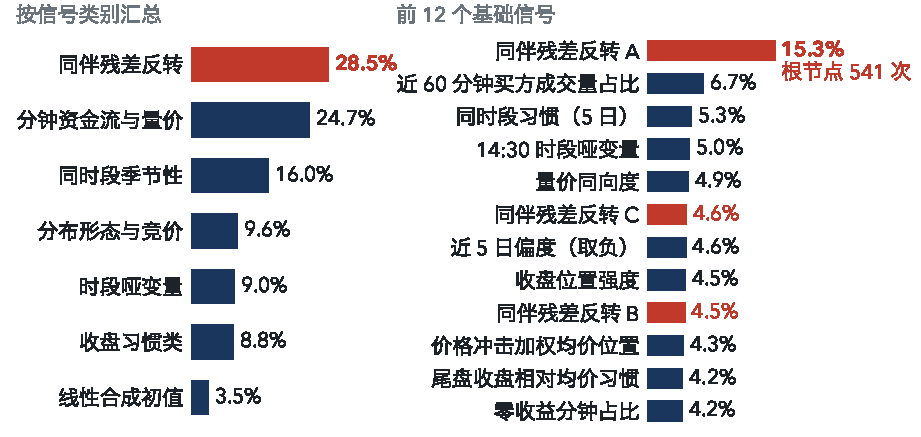
\includegraphics[width=\figwidth]{figures/fig_tree_importance_r.pdf}
\source{比赛平台分钟行情，团队计算}
\end{figure}

图表~\ref{fig:importance} 中权重第二大的一类是分钟资金流与量价，它们与同伴残差反转是同一机制在不同尺度上的表现：短时间内集中的买入压力推高价格，随后部分回吐。近 60 分钟上涨分钟的成交量占总成交量的比例越高，股票随后越弱，这一信号单独使用时 2020–2024 年逐年 RankIC 为 −0.0760、−0.0719、−0.0597、−0.0617、−0.0451。量价同向度方向同样为负，反映放量推动的价格变动随后回吐。

\subsection{个股在固定时段的收盘习惯逐日重复}\label{sec:flow}

图表~\ref{fig:importance} 中权重第三的一类是同时段季节性。个股在一天中某个半小时收在均价之上还是之下，会在之后的交易日重复出现。我们用下一个半小时段“段收盘价 ÷ 段均价 − 1”的过去 10 日均值度量这一习惯，它与标签的形式相同。该信号 2020–2024 年逐年单独 RankIC 为 0.0119、0.0122、0.0157、0.0216、0.0169，与早期反转类主信号的相关系数只有 0.01，对其取残差后的 RankIC 为 0.0276，提供了反转之外的独立信息。5 日窗口的同类信号在单个信号的分裂权重中排第三，占 5.3\%。

收盘习惯类是习惯类信号中变化最慢的一组。尾盘收盘相对均价习惯与收盘位置强度都按过去 20 日计算，日内不变，几乎不贡献换手；前者在 14:30 截面的单独 RankIC 为 0.066，在其他截面约为 0。两者合计占分裂权重的 8.8\%，在树中与反转、资金流信号共同决定分裂，起条件修正的作用。

\subsection{挂单笔数与单笔规模预示相反的方向}\label{sec:orderbook}

常规的盘口不平衡只看挂单量。同样的买一挂单量，可能由多笔小单构成，也可能由少数大单构成（图表~\ref{fig:book} 左）：前者更接近分散的真实需求，后者更可能是压盘或做市挂单。只看挂单量，无法区分这两种情形。

我们把挂单笔数与单笔挂单规模分开计算。在五个不同的统计窗口上，一档笔数失衡（买方笔数减卖方笔数，再除以两者之和）单独 RankIC 为 +0.022～+0.051，五个窗口均为正向；一档单笔规模比（买方与卖方平均单笔挂单规模之比的对数）单独 RankIC 为 −0.019～−0.036，五个窗口均为反向（图表~\ref{fig:book} 右）。两者方向相反，且在各窗口一致，说明同一挂单量中包含方向相反的两部分信息。

\begin{figure}[htbp]
\caption{同样的挂单量，委托结构不同（左，示意）；笔数与单笔规模的单独 RankIC 方向相反（右）}\label{fig:book}
\centering
\begin{minipage}[c]{0.40\textwidth}\centering
\begin{tikzpicture}[x=1cm,y=1cm]
  \draw[rgrey,line width=0.6pt] (0,2.55) -- (0,0) -- (1.9,0) -- (1.9,2.55);
  \foreach \i in {0,1,2} \foreach \j in {0,1,2,3}
    \draw[rline,line width=0.6pt] (0.14+0.55*\i,0.1+0.6*\j) rectangle ++(0.5,0.5);
  \draw[rgrey,line width=0.6pt] (2.9,2.55) -- (2.9,0) -- (4.8,0) -- (4.8,2.55);
  \draw[rnavy,line width=0.6pt] (3.04,0.1) rectangle (4.66,1.2);
  \draw[rnavy,line width=0.6pt] (3.04,1.3) rectangle (4.66,2.4);
  \draw[rgrey,line width=0.6pt,decorate,decoration={brace,amplitude=4pt}] (0,2.7) -- (4.8,2.7);
  \node[note,anchor=south] at (2.4,2.85) {买一挂单量相同};
  \node[note] at (0.95,-0.35) {多笔小单};
  \node[note] at (3.85,-0.35) {少数大单};
  \draw[flow,draw=raccent] (0.6,-1.45) -- (0.6,-0.8);
  \node[note,anchor=west,text=raccent] at (0.75,-1.12) {随后偏强};
  \draw[flow] (3.5,-0.8) -- (3.5,-1.45);
  \node[note,anchor=west] at (3.65,-1.12) {随后偏弱};
\end{tikzpicture}
\end{minipage}\hfill
\begin{minipage}[c]{0.56\textwidth}\centering
{\tablesetup
\begin{tabularx}{\linewidth}{@{}L P{3.0cm} P{1.9cm}@{}}
\toprule
信号 & 单独 RankIC & 方向一致的窗口\\
\midrule
一档笔数失衡 & +0.022～+0.051 & 5 个，正向\\
一档单笔规模比 & −0.019～−0.036 & 5 个，反向\\
\bottomrule
\end{tabularx}}
\end{minipage}
\source{团队整理；比赛平台分钟行情，团队本地评测}
\end{figure}

最终因子取截面前 10 分钟的一档平均委托规模比，取负并做跨截面平滑（系数 0.3），以 0.30 的权重加入，是权重最大的增量信号。它的权重来自一次大范围的筛选：约 200 个覆盖五年数据的候选逐个以 0.1 的权重加到基础组合上，只有委托结构类信号能使 RankIC、ICIR、多空组合夏普比率、压力稳定性四项同时上升且换手率不升。

订单流提供了另一种委托信息。截面前 10 分钟的主动买卖失衡单独使用时五年 RankIC 只有 0.0007，各年正负交替；以 0.15 的权重加入组合后，ICIR 提高 0.036，压力稳定性提高 0.028。单独使用时，它的作用被反转效应掩盖，控制反转之后才表现出延续性。它与取负使用的最后 10 分钟签名成交量并不矛盾：前者按成交价在买卖价之间的位置判断订单本身的方向，后者用分钟 K 线实体度量价格已被推动的程度。

\subsection{收盘集合竞价使 14:30 截面另有规律}\label{sec:1430}

在基础组合中，14:30 是唯一被明显区别对待的截面。在 2024 年，基础组合在 14:30 截面的 RankIC 为 0.109，14:00 为 0.061，其余截面为 0.074～0.082；14:30 的时段哑变量从不出现在根节点，只出现在树的第 1～4 层。原因在于标签：14:30 截面的窗口末价是收盘集合竞价价（图表~\ref{fig:timeline}）。

我们在 14:30 截面上发现三条只在该截面成立的规律。一是收盘竞价收益有惯性，1 日、5 日、20 日三个窗口的版本方向一致；作为对照，午休没有集合竞价，“11:30 至午后开盘”的惯性没有预测力。二是截面前的盘口压力在收盘竞价中回吐：一档委托规模比、段末委托结构、主动买卖失衡在 14:30 的单独 RankIC 分别为 +0.0029、+0.0130、−0.0136，其中只有主动买卖失衡在 14:30 无条件为负。反向调整的主要作用是抵消全时段版本在 14:30 带来的正向载荷，属于组合中的条件效应。三是当天成交越放量，股票在 14:30 之后越倾向于上涨至收盘，与放量信号在全天平均的方向相反。收盘价是指数、基金净值与机构考核的基准，收盘竞价因而存在稳定的买卖不平衡来源，这是上述三条规律的一个经济解释。

时段专用的信号容易拟合噪声：每为一个时段单独设定信号，就多出一组自由度，候选越多，越容易把偶然结果当成时段规律。因此我们先检验 14:30 是否确实特殊（图表~\ref{fig:placebo}）。把四个增量信号分别改为只在 10:00 至 14:00 六个截面中的一个生效，权重 ±0.20，共 48 组；相对对照，RankIC 变化的均值为 −0.00019，标准差为 0.00017，最大为 +0.00015。放量信号另做 60 组，结果同样在误差范围内。加入 14:30 反向调整项一步的 RankIC 增量为 +0.0012，约为上述标准差的 7 倍。

\begin{figure}[htbp]
\caption{增量信号改在其余六个截面生效的 48 组对照均在 ±0.0005 以内，14:30 反向调整项为 +0.0012（本地 2023–2024）}\label{fig:placebo}
\centering
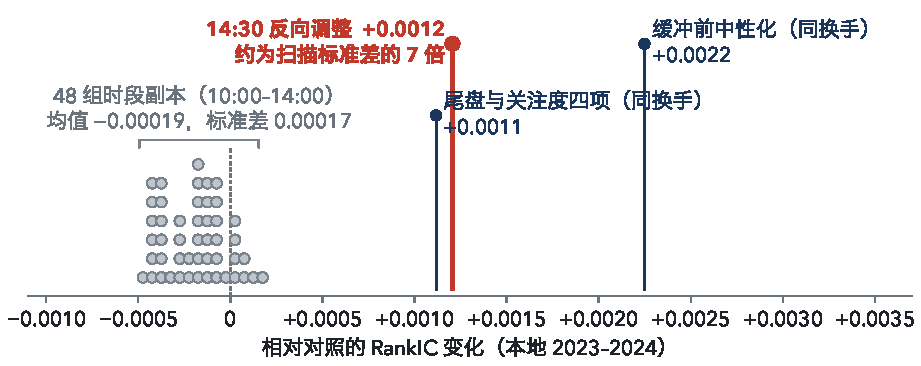
\includegraphics[width=\figwidth]{figures/fig_slot_placebo_r.pdf}
\source{比赛平台分钟行情，团队本地评测}
\end{figure}

\subsection{关注度消退与上午的日内锚定}\label{sec:attention}

最后一类是关注度与日内锚定。成交额放大往往伴随关注度冲击，之后关注度回落，价格回吐关注带来的溢价。我们用约一周相对约一个月的成交额放大程度度量这一过程，取负后单独使用的五年 RankIC 为 0.0137，换手率只有 0.047。它与 14:30 的放量后继续上涨并不矛盾：前者基于多日成交额、变化缓慢，后者是当日变量，且只在包含收盘竞价的窗口成立。日内锚定指开盘后的冲高或下探在上午向 10:00 的价格回吐。这一信号只在 10:30、11:00、11:30 三个截面使用，单独使用的五年 RankIC 为 0.0733、ICIR 为 1.231，换手率为 0.378。

单独 RankIC 的高低并不决定一项信号在组合中的价值：主动买卖失衡单独使用时 RankIC 接近 0，在组合中却提高了 ICIR；尾盘反转类单独 RankIC 较高，换手率也高达 0.74～0.86。因此，增量信号按加入完整计算流程后五项指标是否改善来筛选（第~\ref{sec:linear}~节），各项单独使用时的逐年 RankIC 见附录 G。

这些信号单独使用都不强，适用截面也各不相同。第~\ref{sec:ch3}~章讨论如何把它们组合成一个因子。

% ==================================================================
\section{浅层树组合基础信号，新信息逐项叠加}\label{sec:ch3}

组合方式取决于信号的性质：反转信号与标签之间是非线性关系，固定的线性权重无法表达；新发现的信息各有适用时段，需要逐项单独检验。因此我们采用两种组合方式。27 个基础信号由 16 个浅层梯度提升树组合后取平均，模型只在 2020–2022 年拟合；在样本外的 2023、2024 年，RankIC 比同输入的线性合成分别高 0.0095 和 0.0086。基础组合之外的新信息作为 15 项增量信号，以小权重逐项线性叠加，每一项都可以单独剔除和检验。树的代价是换手率升至 0.518。

\subsection{基础组合由 16 个浅层树平均而成}\label{sec:tree}

线性合成把每个信号的作用固定为一个权重，无法表达大涨大跌与小涨小跌之后回补方式不同这类非线性。为在控制过拟合的前提下刻画这种非线性，我们选用浅层梯度提升树，并对多个随机种子的模型取平均（图表~\ref{fig:ensemble}）。基础组合包含三种配置：深度 4、150 棵树，4 个随机种子；深度 4、130 棵树，4 个随机种子；深度 5、100 棵树，8 个随机种子。16 个模型共 1920 棵树，全部等权平均，不挑选随机种子。模型只在 2020 年 1 月 1 日至 2022 年 12 月 31 日的数据上拟合，2023、2024 两年为样本外。

\begin{figure}[htbp]
\caption{基础组合的结构（每个小方块代表一个随机种子的模型）}\label{fig:ensemble}
\centering
\begin{tikzpicture}[x=1cm,y=1cm]
  \node[node] (in) at (0,0) {27 个基础信号\\每列 32 箱};
  \foreach \y/\lab/\n in {0.9/{深度 4，150 棵}/4, 0/{深度 4，130 棵}/4, -0.9/{深度 5，100 棵}/8} {
    \node[note,anchor=west] at (2.85,\y) {\lab};
    \foreach \i in {1,...,\n}
      \draw[rnavy,line width=0.6pt] (6.05+0.45*\i-0.45,\y-0.16) rectangle ++(0.32,0.32);
    \draw[flow] (in.east) -- (2.75,\y);
    \draw[flow] (9.6,\y) -- (10.35,0);
  }
  \node[key] (avg) at (10.9,0) {平均};
  \node[node,right=5mm of avg] (out) {基础组合\\输出};
  \draw[flow] (avg) -- (out);
  \node[soft,dashed] (tgt) at (6.6,-2.25) {训练目标：标签截面秩\\$+\,w\,\times$ 之后两个截面标签之和的截面秩};
  \draw[flow,draw=rgrey,dashed] (tgt.north) -- (6.6,-1.15);
  \node[note,anchor=west] at ([xshift=4mm]tgt.east) {$w=0.25$（深度 4）\\$w=0.40$（深度 5）};
  \node[note,anchor=east] at ([xshift=-4mm]tgt.west) {拟合区间\\2020–2022 年};
\end{tikzpicture}
\source{团队整理}
\end{figure}

训练目标在标签的截面秩上加入多周期辅助项：
\begin{equation}
\tilde y_{i,t}=\operatorname{rank}_t\!\left(y_{i,t}\right)+w\cdot\operatorname{rank}_t\!\Big(\sum_{k=1}^{2}y_{i,t+k}\Big),
\end{equation}
其中 $\operatorname{rank}_t$ 表示截面秩，$t+1$、$t+2$ 是同一交易日之后的两个截面，深度 4 的模型取 $w=0.25$，深度 5 的模型取 $w=0.40$。辅助项使树偏向持续时间更长的信号；它只改变训练目标，推理时不使用模型此前的任何输出。

为控制过拟合，每个输入按拟合期的分位数分为 32 箱，分箱边界写入模型；行抽样比例 8\%，列抽样比例 80\%，叶子节点至少包含 3000 个样本，L2 正则系数 200，学习率 0.06。比赛平台未提供 sklearn 与 LightGBM，树用 numpy 实现，以 JSON 格式嵌入因子代码，推理时不重新拟合。全部参数见附录 C。

\subsection{浅层树在样本外两年与公榜均优于线性合成}\label{sec:treeoos}

图表~\ref{fig:treelin} 比较同一批基础信号下浅层树组合与线性合成的表现。在本地样本外的 2023 年，浅层树的 RankIC 高 0.0095，ICIR 高 0.131，压力稳定性高 0.141；2024 年分别高 0.0086、0.127、0.074。两者同时提交公榜时，浅层树的 RankIC 高 0.0056，ICIR 高 0.282，多空组合夏普比率高 8.60，压力稳定性高 0.236，换手率高 0.134。

\begin{figure}[htbp]
\caption{同一批基础信号下，浅层树组合在样本外两年与公榜的 RankIC、ICIR 均高于线性合成}\label{fig:treelin}
\centering
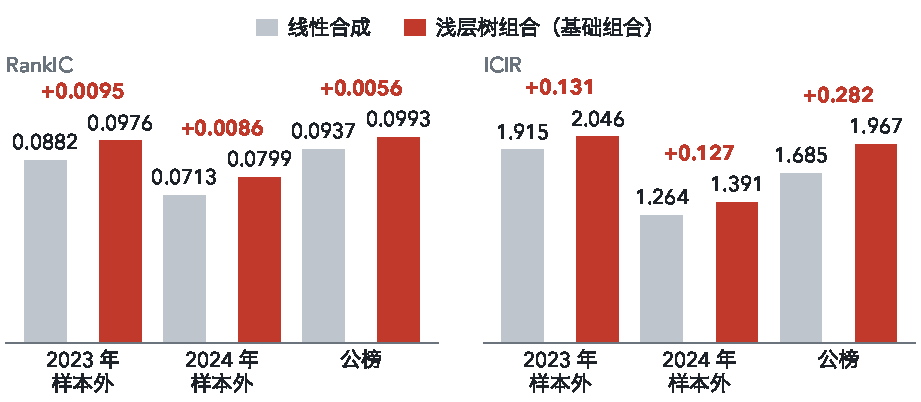
\includegraphics[width=\figwidth]{figures/fig_tree_vs_linear_r.pdf}
\source{比赛平台分钟行情，团队本地评测；比赛平台公榜，团队整理}
\end{figure}

这一结果在不同设定下方向不变。更换随机种子、去掉时段哑变量、只用 2021–2022 年拟合、把树的规模减半，样本外增益都没有改变符号；去掉时段哑变量后，增益缩小到原来的三分之一至二分之一。我们还直接测量了样本内的高估幅度：同一树方法把 2020 年由样本内改为样本外后，RankIC 增量由 +0.00460 降至 +0.00303（−34\%），ICIR 增量由 +0.1014 降至 +0.0682（−33\%），没有改变符号。换手方面，2023、2024 年浅层树的换手率分别比线性合成高 0.144 和 0.141，本地 2023–2024 年合计为 0.518，线性合成约为 0.38。

\subsection{树的增益来自反转信号的非线性}\label{sec:nonlinear}

树的增益可能来自信号之间的交互，也可能来自单个信号的非线性，我们用两组检验区分这两种来源。第一组在同一样本切分下，用 15 个分量加 4 个交互项做岭回归，2023、2024 年相对线性解的 ICIR 只提高 0.0212 和 0.0014，同一组对照中梯度提升树提高 0.0482 和 0.0078，交互项不能解释树的增益。

第二组是单调约束检验（单个深度 4 模型、单随机种子）。只对反转信号不加约束、其余信号按经济方向约束为单调时，RankIC 只下降 0.0003～0.0008，ICIR 与压力稳定性略有上升，换手率下降。由此判断，非线性集中在反转信号上，大涨大跌与小涨小跌之后的回补方式不同；其余信号大体按经济方向单调地起作用，它们在树中的非单调部分多为噪声，还使换手率增加约 0.025。

\subsection{新信息以增量信号线性叠加，不作为树的输入}\label{sec:linear}

既然浅层树优于线性合成，自然的做法是把新发现的信息也作为树的输入。我们做了这一实验：把全部增量信号与委托规模比加入树的输入，未加换手控制时 RankIC 提高约 0.005、ICIR 提高约 0.14，但换手率由 0.52 升至 0.585；用缓冲带把换手率控制在约 0.29 之后，五项为 RankIC 0.0908、ICIR 1.758、多空组合夏普比率 46.77、压力稳定性 1.606、换手率 0.291，低于浅层树加线性增量信号的 0.0920、1.801、48.03、1.659、0.289。深度 5、6 的树（8 个随机种子平均）同样没有改善。原因是树从新信息中获得的 RankIC 主要来自相邻截面之间变化快的成分，经过换手控制后无法保留；线性增量信号是在换手控制的口径下筛选的，变化较慢。

增量信号的叠加方式是：每一项先逐截面排名并标准化，再按
\begin{equation}
z_t\leftarrow\operatorname{std}_t\!\big(z_t+w_j\cdot\operatorname{std}_t(x_{j,t})\big)
\end{equation}
叠加到当前合成信号 $z_t$ 上，其中 $x_{j,t}$ 是第 $j$ 项增量信号，$w_j$ 是其权重，$\operatorname{std}_t$ 表示截面标准化；每加一项重新标准化一次。权重只取 0.10、0.15、0.20、0.30、−0.20 几个固定档位。筛选标准是加入完整计算流程后五项指标是否改善，不看单独 RankIC。尾盘与关注度四项（第~\ref{sec:slot1430}~节）的权重放大到 1.5 倍、2 倍后，在相同换手率下五项都不如原权重 0.10。

15 项增量信号中，7 项在全部截面起作用，7 项只在 14:30 起作用，1 项只在 10:30、11:00、11:30 起作用；生效截面、权重与方向见附录 B。


\subsection{14:30 专用信号与尾盘、关注度四项的增量}\label{sec:slot1430}

第~\ref{sec:1430}~节的三条 14:30 规律分别转化为三组专用增量信号：收盘竞价惯性的 20 日、5 日两个版本，权重各 +0.20；一档委托规模比、段末委托结构、主动买卖失衡三项全时段信号在 14:30 的反向调整项，权重各 −0.20；本段放量与当日至今放量两项，权重各 −0.20，作用于取负后的放量信号，净效果是当天越放量，因子值越高。图表~\ref{fig:steps1430} 显示，14:30 截面的 RankIC 随三组信号依次加入，由 0.105 升至 0.110、0.117～0.119，最后达到 0.128～0.130，累计提高约两成。

\begin{figure}[htbp]
\caption{三组 14:30 专用信号使该截面 RankIC 由 0.105 升至 0.128～0.130（本地 2023–2024）}\label{fig:steps1430}
\centering
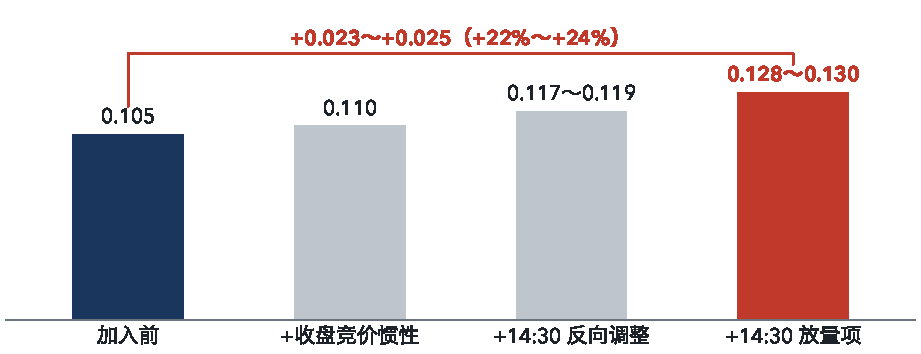
\includegraphics[width=0.84\figwidth]{figures/fig_1430_steps_r.pdf}
\source{比赛平台分钟行情，团队本地评测}
\end{figure}

最后加入的是尾盘与关注度四项：最后 10 分钟签名成交量占本段的比例、最后 10 分钟收益、成交额消退、上午相对 10:00 的回吐。它们以上一版因子为基础，从 255 个候选中逐个重新筛选得到。在换手率约 0.29 的同一水平上，四项合计使 RankIC 提高 0.0011，ICIR 提高 0.012，多空组合夏普比率提高 0.25，压力稳定性提高 0.016，换手率降低 0.001，五项全部改善。

浅层树与增量信号提高了 RankIC，但树也使换手率升高，而公榜综合得分对换手率敏感。

% ==================================================================
\section{在评测使用的排名上控制换手}\label{sec:ch4}

降低换手不能以削弱信号为代价，因此只应减少无效调仓。换手只发生在多空组合的名单边界，因此换手缓冲带只处理边界附近股票的进出，输出值只做最小幅度调整。平台按剔除风格与行业后的排名划分名单，缓冲带相应放在基于前一交易日暴露的风格与行业中性化之后。从基础组合到最终因子，换手率由 0.518 降至 0.290，RankIC 提高 0.0038，ICIR 提高 0.144，代价是多空组合夏普比率下降 2.59。

\subsection{换手只在名单边界处产生}\label{sec:boundary}

换手率只计多头组合与空头组合的成分替换，名单内部的排序变化不计入，因此控制换手的对象是名单边界附近的股票，无需平滑全部股票的输出。两种做法的对照支持这一判断：在相近的换手率下，缓冲带（换手率 0.359）的 RankIC 为 0.0824、ICIR 为 1.580、多空组合夏普比率为 46.25、压力稳定性为 1.486；日内平滑（换手率 0.367）分别为 0.0825、1.554、48.46、1.459。两者 RankIC 持平，缓冲带的 ICIR 与压力稳定性更高，日内平滑的多空组合夏普比率更高。

换手也并非越低越好。同一组因子用整体加分的缓冲带把公榜换手率由 0.39 依次降至 0.29、0.24、0.20，四项质量指标逐档下降：换手率降至 0.24 时，公榜 RankIC 由 0.0952 降至 0.0855，ICIR 由 1.862 降至 1.592，多空组合夏普比率由 55.81 降至 43.38，压力稳定性由 1.868 降至 1.525，公榜得分随之下降。

\subsection{缓冲带决定名单归属，最小幅度调整决定输出值}\label{sec:buffer}

换手缓冲带（hysteresis）在同一交易日内按截面顺序执行。记截面 $t$ 中性化后的标准分为 $z_{i,t}$，上一截面的名单归属为 $s_{i,t-1}\in\{+1,0,-1\}$，分别表示在多头组合、不在名单、在空头组合。划分名单时使用
\begin{equation}
v_{i,t}=z_{i,t}+\beta\, s_{i,t-1},
\end{equation}
$v_{i,t}$ 的截面百分位排名高于 0.9 的股票进入多头组合 $L_t$，不高于 0.1 的进入空头组合 $S_t$。上一截面已在名单内的股票因此获得 $\beta$ 个标准差的保留优势，排名小幅回落时仍留在名单内；名单外的股票需要明显超过它才能换入（图表~\ref{fig:buffer} 左）。09:30 截面清空名单记录，10:00 是每天第一个计分截面，不使用缓冲。最终因子取 $\beta=1.1$。

名单确定之后，输出值的调整方式决定了评测使用的排名。常见的整体加分做法把名单内全部股票的得分加上 $\beta$，名单内外的距离与排序随之改变。我们采用最小幅度调整（图表~\ref{fig:buffer} 右），输出为
\begin{equation}
\hat z_{i,t}=\begin{cases}
\max\big(z_{i,t},\ \max_{j\notin L_t} z_{j,t}+m\big), & i\in L_t,\\[2pt]
\min\big(z_{i,t},\ \min_{j\notin S_t} z_{j,t}-m\big), & i\in S_t,\\[2pt]
z_{i,t}, & \text{其他},
\end{cases}
\end{equation}
即多头名单内低于“名单外最高者 $+\,m$”的股票调整到该值，空头组合对称处理，其余股票保持原值，被调整的股票之间保持原有次序。最终因子取 $m=0.6$。按这一输出排名时，我们划定的名单恰好位于前、后 10\%，名单内外各自的相对次序不变。间隔 $m$ 在 0.3～1.0 之间效果最好，达到 1.5 以上开始变差，$m=3.0$ 时 RankIC 降至 0.0645；可能的原因是间隔过大时名单内股票成为极端值，这一点未单独检验。

\begin{figure}[htbp]
\caption{换手缓冲带决定名单归属（左），最小幅度调整决定输出值（右）（示意）}\label{fig:buffer}
\centering
\begin{minipage}[t]{0.485\textwidth}\centering
\begin{tikzpicture}[x=1cm,y=1cm]
  \foreach \y/\lab in {0/上一截面,-1.45/无缓冲带,-2.9/有缓冲带} {
    \node[note,anchor=east] at (1.55,\y) {\lab};
    \draw[rline,line width=0.6pt] (1.7,\y) -- (5.1,\y);
  }
  \draw[rgrey,dashed] (3.6,0.3) -- (3.6,-0.3);
  \draw[rgrey,dashed] (3.6,-1.15) -- (3.6,-1.75);
  \draw[rgrey,dashed] (4.2,-2.6) -- (4.2,-3.2);
  \node[note,anchor=south] at (3.6,0.3) {名单分界};
  \draw[flow,draw=rgrey] (5.3,0) -- (6.2,0);
  \node[note,anchor=south] at (5.75,0.05) {得分高};
  \fill[rnavy] (4.1,0) circle (2.6pt); \node[note,anchor=north] at (4.1,-0.08) {A};
  \draw[rnavy,fill=white] (3.0,0) circle (2.6pt); \node[note,anchor=north] at (3.0,-0.08) {B};
  \fill[rnavy] (3.2,-1.45) circle (2.6pt); \node[note,anchor=north] at (3.2,-1.53) {A};
  \draw[rnavy,fill=white] (3.95,-1.45) circle (2.6pt); \node[note,anchor=north] at (3.95,-1.53) {B};
  \node[note,anchor=west] at (5.2,-1.45) {A 换出\\B 换入};
  \draw[rline,fill=white] (3.2,-2.9) circle (2.6pt);
  \draw[flow,draw=raccent] (3.28,-2.78) to[out=40,in=140] (4.52,-2.78);
  \node[note,anchor=south,text=raccent] at (3.9,-2.5) {$+\beta$};
  \fill[raccent] (4.6,-2.9) circle (2.6pt); \node[note,anchor=north] at (4.6,-2.98) {A};
  \draw[rnavy,fill=white] (3.95,-2.9) circle (2.6pt); \node[note,anchor=north] at (3.95,-2.98) {B};
  \node[note,anchor=west] at (5.2,-2.9) {A 保留\\B 未换入};
\end{tikzpicture}
\end{minipage}\hfill
\begin{minipage}[t]{0.505\textwidth}\centering
\begin{tikzpicture}[x=1cm,y=1cm]
  \foreach \y/\lab in {0/原始得分,-1.45/整体加分,-2.9/最小幅度调整} {
    \node[note,anchor=east] at (2.15,\y) {\lab};
    \draw[rline,line width=0.6pt] (2.3,\y) -- (6.85,\y);
  }
  \draw[rgrey,dashed] (4.05,0.3) -- (4.05,-3.15);
  \draw[raccent,dashed] (4.5,0.3) -- (4.5,-3.15);
  \node[note,anchor=south east] at (4.13,0.3) {名单外最高者};
  \node[note,anchor=south west,text=raccent] at (4.42,0.3) {$+\,m$};
  \foreach \y in {0,-1.45,-2.9}
    \foreach \x in {2.5,2.85,3.2,3.55,4.05} \draw[rnavy,fill=white] (\x,\y) circle (2.3pt);
  \foreach \x in {3.8,4.85,5.25,5.65,6.05} \fill[rnavy] (\x,0) circle (2.3pt);
  \foreach \x in {4.4,5.45,5.85,6.25,6.65} \fill[rgrey] (\x,-1.45) circle (2.3pt);
  \draw[flow,draw=rgrey] (3.8,-1.25) -- (4.37,-1.25);
  \node[note,anchor=north west] at (4.62,-1.56) {名单内全部上移};
  \foreach \x in {4.85,5.25,5.65,6.05} \fill[rnavy] (\x,-2.9) circle (2.3pt);
  \fill[raccent] (4.5,-2.9) circle (2.3pt);
  \draw[flow,draw=raccent] (3.8,-2.76) to[out=55,in=125] (4.45,-2.76);
  \node[note,anchor=north west] at (4.62,-3.01) {只调整边界附近};
\end{tikzpicture}
\end{minipage}
\source{团队整理}
\end{figure}

在相同换手率下，最小幅度调整优于整体加分。换手率约 0.26 时，最小幅度调整的 RankIC 为 0.0820、ICIR 为 1.649，整体加分为 0.0766、1.555；换手率 0.36、0.21、0.17 三档的比较结论相同。另一种调整方式是压低名单外股票的得分，采用后 RankIC 降至 0.03～0.05。分时段设定缓冲强度、同时参考前两个截面的名单、按股票自适应缓冲宽度等其他形式，在相同换手率下均不优于统一缓冲强度的最小幅度调整。

缓冲带使用同一交易日内上一截面的多空名单，这是截面 $t$ 之前已经确定的信息。计算在同一次调用内完成，每天 10:00 重置，不依赖跨日状态。缓冲带只决定名单边界附近股票的归属，输出值仍由当前截面的标准分决定。

\subsection{缓冲带放在剔除风格与行业之后}\label{sec:neutral}

早期版本在原始合成得分的排名上划定缓冲名单。平台先剔除风格与行业再排名，两个排名并不相同：一部分被缓冲带保留的股票落在评测名单之外，评测名单边界附近的股票反而没有得到保留，缓冲带的一部分作用落在评测不计分的名单上。改进的做法是在缓冲带之前做一次与评测同口径的中性化（图表~\ref{fig:order}）：逐截面把合成信号对 10 个风格因子与申万一级行业哑变量（含截距）做最小二乘回归，取残差后重新标准化。风格暴露与行业一律取该股票前一交易日的记录，不用当天值；有效样本少于 50 只的截面跳过。

\begin{figure}[htbp]
\caption{缓冲带放在中性化之前与之后的流程对照}\label{fig:order}
\centering
\begin{tikzpicture}[node distance=7mm]
  \node[note,anchor=east] (lab2) at (0,0) {改进后};
  \node[node,right=3mm of lab2] (b1) {原始得分};
  \node[key,right=of b1] (b2) {前一交易日\\中性化};
  \node[node,right=of b2] (b3) {缓冲带\\定名单};
  \node[node,right=of b3] (b4) {平台\\中性化};
  \node[node,right=of b4] (b5) {评测名单};
  \foreach \a/\b in {b1/b2,b2/b3,b3/b4,b4/b5} \draw[flow] (\a) -- (\b);
  \node[note,anchor=east] (lab1) at (0,1.75) {原做法};
  \node[soft] (a1) at (b1 |- lab1) {原始得分};
  \node[soft] (a3) at (b3 |- lab1) {缓冲带\\定名单};
  \node[soft] (a4) at (b4 |- lab1) {平台\\中性化};
  \node[soft] (a5) at (b5 |- lab1) {评测名单};
  \foreach \a/\b in {a1/a3,a3/a4,a4/a5} \draw[flow,draw=rgrey] (\a) -- (\b);
  \draw[rgrey,dashed,line width=0.6pt] ([yshift=3pt]a3.north) -- ++(0,0.25) -| ([yshift=3pt]a5.north);
  \node[note,anchor=south] at ($([yshift=3pt]a3.north)!0.5!([yshift=3pt]a5.north |- a3.north)+(0,0.3)$) {两个排名不同};
  \draw[raccent,line width=0.7pt] ([yshift=-3pt]b3.south) -- ++(0,-0.25) -| ([yshift=-3pt]b5.south);
  \node[note,anchor=north,text=raccent] at ($([yshift=-3pt]b3.south)!0.5!([yshift=-3pt]b5.south |- b3.south)+(0,-0.3)$) {两个排名基本一致};
\end{tikzpicture}
\source{团队整理}
\end{figure}

效果在相同换手率下比较。换手率同为 0.357 时，RankIC 由 0.0899 升至 0.0921（+0.0022），ICIR 由 1.777 升至 1.799，多空组合夏普比率提高 2.3，压力稳定性基本持平（−0.001）；2023、2024 两年的 RankIC 都提高约 0.002。这一增量约为时段对照标准差（0.00017）的 12 倍。中性化之后，同一缓冲强度下的换手率由 0.357 降至 0.254；我们把缓冲强度由 1.2 降至 0.7，使换手率回到 0.357，与改动前相同。

这一改进在公榜上同样有效。整体加分的缓冲强度越大，公榜 ICIR 与本地 ICIR 的比值越低，由无缓冲时的 1.186 降至缓冲最强时的 1.002；中性化之后，换手率 0.237～0.357 的四个版本，这一比值都在 1.141～1.152，接近无缓冲的水平。

中性化只用前一交易日的暴露，因此没有利用评测口径的一个性质。平台用当天的风格暴露做中性化，而当天暴露的日变化与当天收益高度相关（规模 0.98、账面市值比 −0.78），在前一交易日的风格暴露上反向加载，可以借助未来信息提高 RankIC。这类做法使用了截面之后的信息，我们记录了这一性质，但没有采用。

\subsection{按换手与 RankIC 的权衡选定缓冲强度}\label{sec:tradeoff}

图表~\ref{fig:tradeoff} 左栏比较三组缓冲带的换手率与 RankIC 的关系。每降低 0.1 换手率，整体加分的缓冲带损失约 0.0066 RankIC，中性化后的最小幅度调整损失约 0.0018，约为前者的四分之一；两组的增量信号不完全相同，此处比较的是斜率，并非严格的消融实验。右栏是公榜上同一基础组合、整体加分缓冲强度不同的 7 个因子：公榜换手率由 0.48 降至 0.20，ICIR 由 1.964 降至 1.497，压力稳定性由 1.929 降至 1.423；这 7 个因子的公榜得分在换手率 0.39 处最高，换手更低时随之下降。

\begin{figure}[htbp]
\caption{中性化后的最小幅度调整使每降低 0.1 换手率的 RankIC 损失由 0.0066 降至 0.0018}\label{fig:tradeoff}
\centering
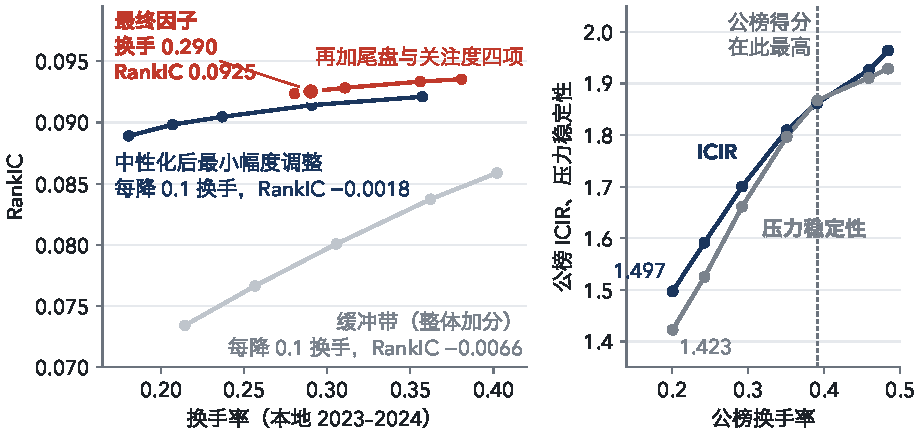
\includegraphics[width=\figwidth]{figures/fig_turnover_tradeoff_r.pdf}
\source{比赛平台分钟行情，团队本地评测；比赛平台公榜，团队整理}
\end{figure}

缓冲强度按目标换手率确定。加入尾盘与关注度四项后，$\beta=1.0$ 时换手率为 0.311，$\beta=1.1$ 时为 0.290，我们取 1.1，使换手率保持在 0.29 左右。中性化口径下，缓冲强度由 1.0 提高到 1.3、换手率由 0.28 降至 0.23 时，公榜同一页面上 RankIC 下降 0.0010，ICIR 下降 0.017，多空组合夏普比率下降 2.75，压力稳定性下降 0.014，公榜得分随之下降；换手率低于 0.28 之后公榜得分不再提高，因此没有继续降低换手率。

\subsection{从基础组合到最终因子的逐步增量}\label{sec:chain}

图表~\ref{fig:chain} 汇总了从基础组合到最终因子的 11 个版本。首尾相比，RankIC 由 0.0888 升至 0.0925（+0.0038），换手率由 0.518 降至 0.290（−0.228，约 −44\%）。各步的缓冲强度不同，单步比较只看图中标出的两组换手率相同的配对，即缓冲前中性化，以及尾盘与关注度四项。

\begin{figure}[htbp]
\caption{从基础组合到最终因子，换手率由 0.518 降至 0.290，RankIC 由 0.0888 升至 0.0925（本地 2023–2024）}\label{fig:chain}
\centering
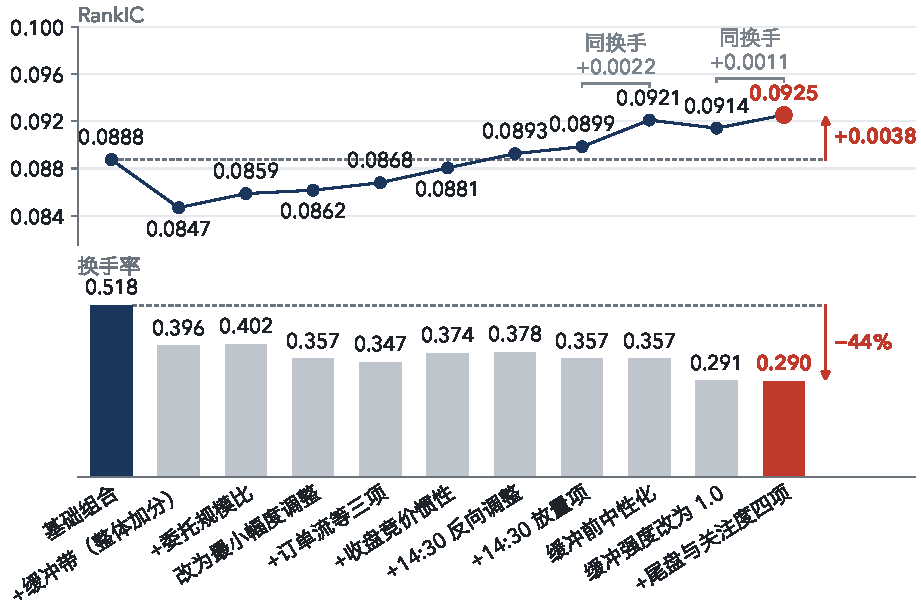
\includegraphics[width=\figwidth]{figures/fig_increment_chain_r.pdf}
\source{比赛平台分钟行情，团队本地评测}
\end{figure}

逐步增量的五项全表见附录 D。从基础组合到最终因子，ICIR 提高 0.144，压力稳定性提高 0.128，多空组合夏普比率下降 2.59；分年看，2023、2024 年 RankIC 分别提高 0.0032 和 0.0043。多空组合夏普比率是五项中对换手最敏感的一项，中性化口径下每降低 0.1 换手率约下降 3～4，上述下降主要来自换手率的降低。


公榜同一页面的分步结果与本地方向一致：浅层树相对线性合成，RankIC 高 0.0056、ICIR 高 0.282；委托规模比与 14:30 反向调整两步，RankIC、ICIR、多空组合夏普比率、压力稳定性都提高；尾盘与关注度四项在低换手、高换手两个作品上五项全部更优，RankIC 分别提高 0.0023 和 0.0025；整体加分的缓冲强度过大、换手率由 0.35 降至 0.24 时，RankIC 下降 0.0076，ICIR 下降 0.218，压力稳定性下降 0.271。

增量信号的权重与缓冲强度都在 2023–2024 年选定。第~\ref{sec:ch5}~章检验这些结论在未参与筛选的年份和私榜上是否成立。

% ==================================================================
\section{结论在样本外是否成立}\label{sec:ch5}

检验分两部分：未参与筛选的 2020–2022 年，以及私榜。基础组合在 2020–2022 年拟合，因此五年检验以线性合成基准为基础组合，加入同一套增量信号与后处理，2020–2024 年每年 RankIC 提高 0.0078～0.0086，未参与筛选的三年与筛选所用的两年相当。私榜上四项质量指标较公榜回落 16\%～28\%，但逐截面 RankIC 的标准差基本不变，换手率由本地 0.290、公榜 0.279 降至私榜 0.266，回落的是信号水平。

\subsection{未参与筛选的三年逐年同向}\label{sec:fiveyears}

浅层树在 2020–2022 年是样本内，不能直接用最终因子做五年检验。我们改用线性合成基准作为基础组合，按最终因子的顺序逐步加入全部增量信号与后处理（图表~\ref{fig:fiveyears}，逐步结果见附录 D）。2020–2024 年 RankIC 依次提高 0.0078、0.0086、0.0082、0.0081、0.0084；ICIR 每年提高 0.196～0.234，压力稳定性每年提高 0.149～0.209，换手率每年降低 0.080～0.098。只有多空组合夏普比率在四个年份下降，与第~\ref{sec:chain}~节换手降低的代价一致。

\begin{figure}[htbp]
\caption{以线性合成基准为基础组合，加入同一套增量信号与后处理后 2020–2024 年每年 RankIC 提高 0.0078～0.0086（本地）}\label{fig:fiveyears}
\centering
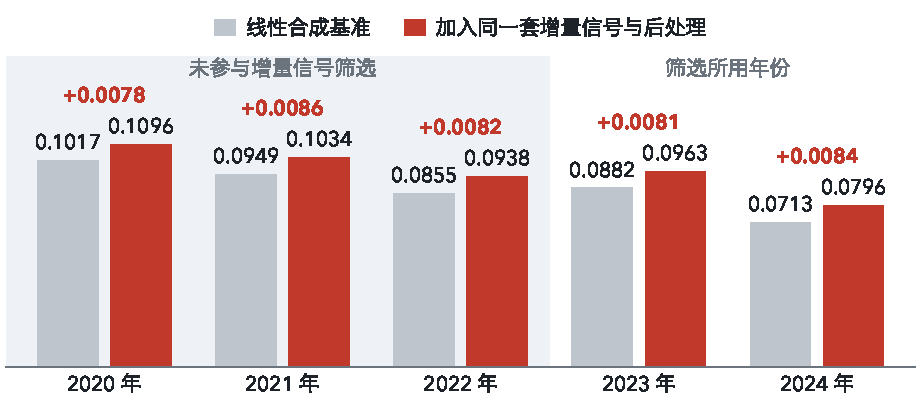
\includegraphics[width=\figwidth]{figures/fig_five_years_r.pdf}
\source{比赛平台分钟行情，团队本地评测}
\end{figure}

加入全部后处理后，五年中每年的 ICIR 都高于 1.4，压力稳定性都高于 1.3。单独检验尾盘与关注度四项，结论相同：它们只在 2023–2024 年筛选，在线性合成基准上 2020–2024 年 RankIC 逐年提高 0.0036、0.0042、0.0030、0.0026、0.0025，ICIR、多空组合夏普比率与压力稳定性五年也都提高。同一套后处理下，浅层树基础组合在 2023、2024 年的 RankIC 比线性合成基准各高 0.0046。在表现最弱的 2024 年，从线性合成（RankIC 0.0713、换手率 0.375）到最终因子（RankIC 0.0842、换手率 0.291），RankIC 提高 0.0129，ICIR 由 1.264 升至 1.541。

\subsection{私榜信号水平回落，波动与换手未变差}\label{sec:private}

图表~\ref{tab:venues} 列出最终因子在本地、公榜、私榜的五项指标。私榜 RankIC 为公榜的 0.768（−23.2\%），四项质量指标较公榜回落 16\%～28\%，换手率则为公榜的 0.953，进一步降低。

\begin{table}[htbp]
\caption{最终因子在本地、公榜、私榜的五项（公榜、私榜为平台原值）}\label{tab:venues}
\centering
{\tablesetup
\begin{tabularx}{\textwidth}{@{}L rrrrr@{}}
\toprule
指标 & 本地 2023–2024 & 本地 2024 & 公榜 & 私榜 & 私榜 ÷ 公榜\\
\midrule
RankIC & 0.0925 & 0.0842 & 0.1028 & 0.0790 & 0.768\\
ICIR & 1.803 & 1.541 & 2.0691 & 1.5593 & 0.754\\
多空组合夏普比率 & 48.50 & 40.82 & 54.1828 & 45.6269 & 0.842\\
压力稳定性 & 1.662 & 1.386 & 1.9532 & 1.4086 & 0.721\\
换手率 & 0.290 & 0.291 & 0.2794 & 0.2662 & 0.953\\
\bottomrule
\end{tabularx}}
\source{比赛平台公榜／私榜，团队整理；比赛平台分钟行情，团队本地评测}
\end{table}

图表~\ref{fig:levelvol} 把回落分解为均值与波动两部分。逐截面 RankIC 的标准差等于 RankIC 除以 ICIR，本地 2023–2024 年约为 0.0513，公榜为 0.0497，私榜为 0.0507，三者几乎相同；压力稳定性与 ICIR 之比，本地为 0.922，公榜为 0.944，私榜为 0.903，较弱的一半截面没有单独恶化。私榜回落的是 RankIC 的均值，信号的波动与换手都没有变差。私榜水平与本地最弱的 2024 年接近：私榜与本地 2024 年之比，RankIC 为 0.938，ICIR 为 1.012，多空组合夏普比率为 1.118，压力稳定性为 1.016。各阶段代表版本的 RankIC 都在 2024 年最低（附录 G），说明 2024 年偏弱是区间本身的特征。

\begin{figure}[htbp]
\caption{私榜 RankIC 均值较公榜下降 23\%，逐截面 RankIC 标准差几乎不变}\label{fig:levelvol}
\centering
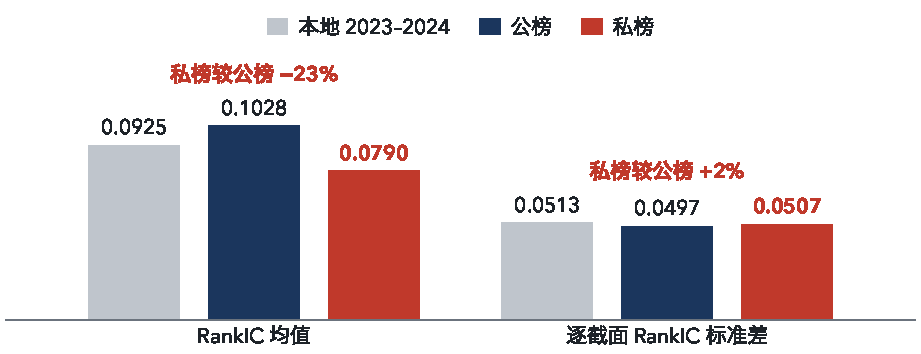
\includegraphics[width=0.84\figwidth]{figures/fig_level_vs_volatility_r.pdf}
\source{比赛平台公榜／私榜，团队整理；比赛平台分钟行情，团队本地评测}
\end{figure}

端到端赛道提供了一个旁证。在同一私榜区间，端到端最终模型（私榜一侧为平台从零重训的模型）的私榜与公榜之比为 RankIC 0.777、ICIR 0.775、压力稳定性 0.769，逐截面 RankIC 标准差同样几乎不变，公榜为 0.0566，私榜为 0.0568。两条构造方法不同的研究路线同幅度回落，更符合私榜区间整体信号偏弱的解释。这一旁证有四点局限：只有一个私榜区间；两个赛道预测同一个标签，研究思路有相互借鉴，不是独立样本；私榜区间的日期未公布；私榜的参评池不同，不能用综合得分比较回落幅度。

样本外检验支持上述做法，但证据强度还取决于研究过程中检验过的候选数量。第~\ref{sec:ch7}~章说明如何控制这一影响，以及结论成立的条件。

% ==================================================================
\section{研究方法与结论边界}\label{sec:ch7}

比赛期间我们在本地评测系统上运行了 6600 个评测任务，候选越多，把偶然结果当成规律的风险越大。我们用同一套验证流程筛选每一项改动：准入标准、截断重算、五年逐年与时段对照、公榜事后检验，最终 2 个作品进入私榜。最终因子有五项做法与常规做法不同，其适用条件均以本次评测口径为前提。对实际应用影响最大的局限是尚未完成的交易成本回测与容量分析。

\subsection{每项改动经过同一套验证流程}\label{sec:process}

图表~\ref{fig:validation} 是增量信号与后处理的验证流程。一项改动先在本地评测系统上与对照比较，准入标准是 RankIC、ICIR、多空组合夏普比率、压力稳定性四项不变差，换手率不升，至少一项明显更好，2023、2024 两年分别判定。通过之后，新信号须做截断重算，确认只用截面之前的数据能得到同样的结果；再做五年逐年检验，时段专用的信号另做时段对照；最后提交公榜，只与同一页面上的对照比较。任何一步不通过，改动即停用。

\begin{figure}[htbp]
\caption{增量信号与后处理的验证流程}\label{fig:validation}
\centering
\begin{tikzpicture}[node distance=5mm]
  \node[node] (v1) {本地评测\\平台同口径};
  \node[node,right=of v1] (v2) {准入标准\\两年分别判定};
  \node[node,right=of v2] (v3) {截断重算\\只用截面前};
  \node[node,right=of v3] (v4) {五年逐年\\时段对照};
  \node[node,right=of v4] (v5) {公榜检验\\同页面对照};
  \node[key,right=of v5] (v6) {采用};
  \foreach \a/\b in {v1/v2,v2/v3,v3/v4,v4/v5,v5/v6} \draw[flow] (\a) -- (\b);
  \node[note,anchor=south] at ($(v1.north)!0.5!(v2.north)+(0,0.12)$) {约 200、255、511 组候选};
  \node[note,anchor=south] at ($(v4.north)+(0,0.12)$) {48 + 60 组时段对照};
  \foreach \n in {v2,v3,v4} \draw[flow,draw=rgrey] (\n.south) -- ++(0,-0.55);
  \draw[rline,line width=0.6pt] ([yshift=-16.5mm]v2.center) -- ([yshift=-16.5mm]v4.center);
  \node[note,anchor=north] at ([yshift=-17mm]v3.center) {不通过即停用};
  \node[note,anchor=north] at ([yshift=-2mm]v6.south) {2 个作品\\进入私榜};
\end{tikzpicture}
\source{团队整理}
\end{figure}

本地评测任务按任务编号去重共 6600 个，其中直接评测因子值的任务 4317 个、运行平台代码的任务 2280 个，单日最多 937 个；分配的因子编号 1390 个，最终进入私榜的 2 个。6600 是评测任务数，包含同一候选的重复评测与不同区间的评测，不等于独立假设的个数。为控制选择偏差，我们采取了五项措施：筛选只用 2023–2024 年，并以五年逐年方向一致作为准入条件；公榜只作事后检验；权重只取 0.10、0.15、0.20、0.30、−0.20 几个固定档位；时段专用信号须先验证只有该时段特殊；浅层树全部配置取平均，不挑选随机种子。

\subsection{稳健性与统计显著性}\label{sec:robust}

图表~\ref{tab:robust} 汇总了稳健性检验，均为同口径的本地评测或公榜同一页面上的比较。

\begin{table}[htbp]
\caption{稳健性检验汇总}\label{tab:robust}
\centering
{\tablesetup
\begin{tabularx}{\textwidth}{@{}P{4.2cm} P{3.4cm} L@{}}
\toprule
检验 & 对象 & 结果\\
\midrule
换随机种子、去掉时段哑变量、只用 2021–2022 拟合、树规模减半 & 浅层树组合 & 样本外增益都不改变符号；去掉时段哑变量后增益缩小到三分之一至二分之一\\
10 个半年分段 & 基础组合 & 相对上一版浅层树，五项不变差的次数依次为 10、10、9、10、10；前 6 个半年为样本内\\
全区间拟合 & 全区间拟合的基础组合 & 公榜三次同页面比较一次略优、两次略差，没有稳定收益；事后检查发现主要特征的有效学习区间仍是 2020–2022 年\\
更强的树加同一后处理 & 新信息进树、深度 5 与 6 & 同换手下均不如浅层树加线性增量信号\\
时段对照 & 增量信号 48 组、放量信号 60 组 & 全部在误差范围内，只有 14:30 特殊\\
权重放大 & 尾盘与关注度四项 ×1.5、×2 & 同换手下五项都变差\\
缓冲带的替代形式 & 自适应宽度、两截面记忆、分时段强度 & 均不优于统一强度的最小幅度调整\\
截断重算 & 各分钟信号与竞价信号 & 全部一致；完整因子的截断重算没有记录\\
\bottomrule
\end{tabularx}}
\source{比赛平台分钟行情，团队本地评测；比赛平台公榜，团队整理}
\end{table}

RankIC 均值的 $t$ 统计量约为 $\mathrm{ICIR}\times\sqrt{N}$，$N$ 为观测数。最终因子本地 2023–2024 年约有 3381 个有效截面，$t$ 约为 105；同日相邻截面的 RankIC 自相关为负（−0.13～−0.33），按每天一个观测（484 天）计算更为保守，$t$ 约为 40，最弱的 2024 年约为 24。

单步增量的显著性要弱得多。把尾盘与关注度四项的五年 RankIC 增量当作五次重复，均值为 +0.0032，按年计算的 $t$ 约为 10；自由度为 4，且年与年之间不独立，这一检验只说明增量的方向是否稳定。若按 255 个候选做最保守的 Bonferroni 校正，自由度为 4 时临界 $|t|$ 约为 13.1，该单步增量未达到临界值；从线性合成基准到全部后处理的完整增量，RankIC 的 $t$ 约为 65.6，超过临界值。因此本报告把单步增量表述为小而稳定、在样本外保持的改进，不作统计意义上的显著性判断。

\subsection{只使用截面之前的信息}\label{sec:noleak}

分钟级因子最容易出现的问题是无意中使用了截面之后的数据。为此我们设定四条约束：多日统计一律错开 1 个交易日；分钟统计只用到截面所在的那一分钟；风格暴露与行业取前一交易日的记录；09:30 截面输出 0。缓冲带使用的上一截面多空名单，同样是截面之前已经确定的信息。

截断重算是验证流程中的固定一步：删去截面之后的数据重新计算，与使用全部数据的结果逐值比对。这一检查曾否定一批高分候选。“日内最高价时段”信号用整天数据计算时 RankIC 为 +0.019，只用截面之前的数据重算后为 −0.035；按整天聚合再用于当天各截面的几类写法共影响约 240 个历史候选，全部停用。进入最终因子的各个分钟信号与竞价信号都单独做过截断重算，结果全部一致；完整因子（含增量信号与缓冲带）的截断重算没有记录。数据范围方面，本地只有 3 档盘口，平台为 5 档，全部代码只使用 1～3 档；因子不读取标签表，不使用外部数据。

\subsection{研究分工与 AI 工具}\label{sec:ai}

研究方向、准入标准、提交作品与私榜选择由团队成员决定，平台上的提交、自测、探测脚本运行与规则问询由团队成员完成；AI 编码代理编写因子代码（4 个同伴残差反转信号由团队成员在 AI 编码代理早期代码的基础上开发）、本地评测系统、实验脚本与研究记录，不接触比赛平台。两个赛道的模型输出与因子值互相隔离：因子代码中不含端到端模型的预测，端到端模型的输入中不含因子值。研究思路有相互借鉴：官方标签定义、09:30 截面缺陷、32 个行业的中性化口径最先在端到端赛道的平台探测中查清，因子赛道沿用。AI 工具的完整使用情况见 AI 工具使用说明。

\subsection{五项做法与常规做法的差别}\label{sec:innov}

第~\ref{sec:ch2}～\ref{sec:ch4}~章的做法中，有五项与常规做法不同，出发点都是第~\ref{sec:ch1}~章核实的评测口径：评测在剔除风格与行业后的排名上计分，换手只计同日相邻截面，14:30 的标签包含收盘集合竞价。图表~\ref{tab:innov} 列出每一项在同一评测口径、同一换手水平下与常规做法的差别，论证分别见第~\ref{sec:neutral}、\ref{sec:buffer}、\ref{sec:orderbook}、\ref{sec:1430}、\ref{sec:linear}~节。

\begin{table}[htbp]
\caption{五项做法与常规做法的对照}\label{tab:innov}
\centering
{\tablesetup
\begin{tabularx}{\textwidth}{@{}P{2.9cm} P{2.7cm} L P{3.0cm}@{}}
\toprule
我们的做法 & 常规做法 & 同口径下的差别 & 适用条件\\
\midrule
缓冲带放在中性化之后 & 在原始得分上缓冲或平滑 & 换手率同为 0.357，RankIC +0.0022、ICIR +0.022 & 评测在残差排名上划分名单\\
最小幅度调整 & 名单内整体加分 & 换手率约 0.26，RankIC 0.0820 对 0.0766，ICIR 1.649 对 1.555 & 评测按排名划分前、后 10\% 名单\\
笔数与单笔规模分开度量 & 只看挂单量不平衡 & 约 200 个候选中只有委托结构类四项上升、换手率不升 & 数据提供逐档委托笔数\\
先验证时段特殊性，再设专用信号 & 各截面使用同一组权重 & 14:30 RankIC 由 0.105 升至 0.128～0.130；其余时段 48 组均在 ±0.0005 内 & 收盘集合竞价制度稳定\\
浅层树与线性增量信号分工 & 全部信号进入同一个模型 & 换手率约 0.29，RankIC 0.0920 对 0.0908，ICIR 1.801 对 1.758 & 新信息变化快，评测对换手计分\\
\bottomrule
\end{tabularx}}
\source{团队整理}
\end{table}

表中的适用条件也是结论的边界，其中两点需要补充说明。评测使用当天的风格暴露，我们只使用前一交易日的暴露，因此缓冲带划定的名单与评测名单只能做到基本一致。浅层树与线性增量信号的分工只在新信息以变化快的成分为主、评测对换手计分的条件下检验过，新信息变化缓慢或评测不计换手的情形没有检验。

\subsection{局限与风险提示}\label{sec:limits}

图表~\ref{tab:limits} 按影响大小列出八项局限、各自影响的结论与已做或未做的检验。

\begin{table}[htbp]
\caption{局限、影响的结论与已做的检验}\label{tab:limits}
\centering
{\tablesetup
\begin{tabularx}{\textwidth}{@{}P{0.4cm} L P{3.4cm} P{4.5cm}@{}}
\toprule
 & 局限 & 影响的结论 & 已做或未做的检验\\
\midrule
1 & 私榜四项质量指标较公榜回落 16\%～28\%，区间日期未公布 & 样本外表现能否持续 & 做了均值与波动分解、五年逐年检验\\
2 & 未做含交易成本的回测与容量分析，未统计跨日换手；空头端受融券约束 & 多空组合夏普比率能否转化为收益 & 未做；多空组合夏普比率只衡量多空两端的区分度\\
3 & 浅层树的样本外只有 2023、2024 两年；权重与缓冲强度在 2023–2024 年选定 & 第~\ref{sec:ch3}、\ref{sec:ch4}~章的增量 & 五年检验基于线性合成基准，与最终因子不同\\
4 & 未做形式化的多重检验校正与自助法置信区间 & 单步增量的显著性 & 按最保守校正，尾盘与关注度四项单步未达临界值，完整增量超过临界值\\
5 & 14:30 的效应依赖收盘集合竞价制度 & 第~\ref{sec:1430}、\ref{sec:slot1430}~节 & 做了时段对照；未做制度变化的情景分析\\
6 & 委托结构类与尾盘类信号的单独 RankIC 逐年减弱 & 增量信号未来的贡献 & 已逐年量化（图表~\ref{fig:decay}）\\
7 & 树的可解释性是间接的 & 第~\ref{sec:nonlinear}~节的机制解释 & 有分裂统计与单调约束检验；单变量偏依赖曲线未完成\\
8 & 每加一项都重新标准化，名义权重不等于有效载荷 & 增量信号权重的解读 & 有效载荷没有分解\\
\bottomrule
\end{tabularx}}
\source{团队整理}
\end{table}

影响最大的是前两项。私榜回落已做均值与波动的分解和五年逐年检验，但仍无法与过拟合完全区分。交易层面，按定义推算，换手率 0.29 对应每 30 分钟多头、空头两端各约 29\% 的成分被替换，每天 6 次同日换手观测；含佣金、印花税与冲击成本的回测和容量分析尚未进行，可以在冻结的因子文件上补做。

风险提示：模型基于 2020–2024 年的历史数据，市场微观结构或收盘集合竞价规则的变化可能使相关信号失效；委托结构类与尾盘类信号的单独 RankIC 逐年减弱；多空组合夏普比率不含交易成本，空头端在 A 股受融券约束，不代表可实现收益。本报告不构成投资建议。

% ==================================================================
\newpage
\section*{附录}\addcontentsline{toc}{section}{附录}

\subsection*{A　基础信号变量表}\addcontentsline{toc}{subsection}{A　基础信号变量表}

图表~\ref{tab:inputs} 列出基础组合的 27 个输入，方向指单独使用时与标签的关系。

{\tablesetup\linespread{1.0}\selectfont\renewcommand{\arraystretch}{1.0}\setlength{\LTpre}{19pt}\setlength{\LTpost}{0pt}
\begin{xltabular}{\textwidth}{@{}P{1.3cm} P{3.1cm} L P{0.9cm} P{1.9cm}@{}}
\caption{基础组合的 27 个输入（进树前均转为截面百分位排名）}\label{tab:inputs}\\
\toprule
记号 & 名称 & 口径 & 方向 & 类别\\
\midrule
\endfirsthead
\multicolumn{5}{@{}l}{\sffamily\footnotesize\color{rgrey}图表~\ref{tab:inputs}（续）}\\[2pt]
\toprule
记号 & 名称 & 口径 & 方向 & 类别\\
\midrule
\endhead
\bottomrule
\endfoot
\bottomrule
\multicolumn{5}{@{}l}{\sffamily\footnotesize\color{rgrey}资料来源：团队整理}\\
\endlastfoot
$x_1$ & 同时段收盘相对均价习惯（10 日） & 下一个半小时段“段收盘价 ÷ 段均价 − 1”的过去 10 日均值，先跨截面平滑再排名 & 正 & 分钟资金流与量价\\
$x_2$ & 价格冲击加权均价位置 & 以 $|r|$ ÷ 成交量加权的当日至今均价，相对当日至今成交量加权均价的偏离 & 正 & 同上\\
$x_3$ & 量价同向度 & $\sum r\cdot(\ln \text{成交量}-\text{此前各分钟均值})\,/\sum|r|$，当日至今 & 负 & 同上\\
$x_4$ & 零收益分钟占比 & 当日至今 & 正 & 同上\\
$x_5$、$x_6$ & 近 60、90 分钟买方成交量占比 & 上涨分钟成交量 ÷ 总成交量 & 负 & 同上\\
$x_7$ & 同伴残差反转 A & 参照价格为上一窗口末价、近 2 与 4 小时均价、昨收，共 16 列 & 正 & 同伴残差反转\\
$x_8$ & 同伴残差反转 B & 在 $x_{10}$ 基础上加一档中间价均值、三档挂单量加权价、微价格偏离、成交价相对中间价 4 个盘口分量，共 56 列 & 正 & 同上\\
$x_9$ & 同伴残差反转 C & 在 $x_8$ 基础上加成交笔数加权价，共 60 列 & 正 & 同上\\
$x_{10}$ & 同伴残差反转 D & 1 小时至约 4 个交易日的 5 个均价与昨收，近 4 小时末价、区间中点、低点的中位数与低振幅加权价，共 40 列；另与低波动、低成交额、低价的排名和按 1 : 0.5 融合 & 正 & 同上\\
$x_{11}$ & 日内已实现峰度（取负） & $n\sum r^4/(\sum r^2)^2$，当日至今 & 正 & 分布形态与竞价\\
$x_{12}$ & 近 5 日已实现偏度（取负） & 最近 1200 分钟 & 正 & 同上\\
$x_{13}$ & 前一日收盘竞价价格冲击 & 前日收盘价 ÷ 前日 14:57 价格 − 1，日内不变 & 正 & 同上\\
$x_{14}$ & 线性合成初值 & 早期反转类主信号的原始值加九个分钟信号的加权排名，取原始值 & 正 & 线性合成初值\\
$x_{15}$～$x_{21}$ & 时段哑变量 & 10:00 至 14:30 七个截面的独热编码 & 由树学习 & 时段\\
$x_{22}$ & 同时段收盘相对均价习惯（5 日） & 同 $x_1$，5 日窗口 & 正 & 同时段季节性\\
$x_{23}$ & 下一时段成交额占比常态 & 下一段成交额占全天比重的过去 20 日均值 & 弱负 & 同上\\
$x_{24}$ & 当日成交节奏相对常态 & 当日至本段累计成交额 ÷ 过去 20 日同一时刻均值 & 负 & 同上\\
$x_{25}$ & 同星期几同时段习惯 & 过去 10 个同星期几的下一段“段收盘价 ÷ 段均价 − 1”均值 & 正 & 同上\\
$x_{26}$ & 尾盘收盘相对均价习惯 & (14:30, 15:00] 段“收盘价 ÷ 均价 − 1”的过去 20 日均值，日内不变 & 正 & 收盘习惯类\\
$x_{27}$ & 收盘位置强度 & 当日收盘价 ÷ 当日 8 个半小时段收盘价最高者 − 1 的过去 20 日均值，日内不变 & 正 & 收盘习惯类\\
\end{xltabular}}

\subsection*{B　增量信号表}\addcontentsline{toc}{subsection}{B　增量信号表}

图表~\ref{fig:slots} 按类别标出 15 项增量信号的生效截面：委托结构与订单流、尾盘反转、关注度消退三组共 7 项在全部截面起作用，上午回吐只在 10:30、11:00、11:30 起作用，其余三组共 7 项只在 14:30 起作用；14:30 一列中的空心点表示与全时段版本方向相反的调整项。
\begin{table}[H]
\caption{15 项增量信号的生效截面}\label{fig:slots}
\centering
\begin{tikzpicture}[x=1cm,y=1cm]
  \foreach \c/\t in {1/10:00,2/10:30,3/11:00,4/11:30,5/13:30,6/14:00,7/14:30}
    \node[note] at (4.45+1.12*\c,0.58) {\t};
  \foreach \r/\lab in {1/委托结构与订单流（3 项）,2/尾盘反转（3 项）,3/关注度消退（1 项）,4/上午回吐（1 项）,5/收盘竞价惯性（2 项）,6/14:30 反向调整（3 项）,7/14:30 放量（2 项）}
    \node[anchor=east,font=\sffamily\small] at (4.9,0.55-0.55*\r) {\lab};
  \foreach \r in {1,2,3} \foreach \c in {1,...,7}
    \fill[rnavy] (4.45+1.12*\c,0.55-0.55*\r) circle (3pt);
  \foreach \c in {2,3,4} \fill[rnavy] (4.45+1.12*\c,0.55-0.55*4) circle (3pt);
  \foreach \c in {1,5,6,7} \fill[rline] (4.45+1.12*\c,0.55-0.55*4) circle (1.4pt);
  \foreach \r in {5,6,7} \foreach \c in {1,...,6} \fill[rline] (4.45+1.12*\c,0.55-0.55*\r) circle (1.4pt);
  \fill[rnavy] (4.45+1.12*7,0.55-0.55*5) circle (3pt);
  \draw[raccent,line width=0.9pt,fill=white] (4.45+1.12*7,0.55-0.55*6) circle (3pt);
  \fill[rnavy] (4.45+1.12*7,0.55-0.55*7) circle (3pt);
  \node[note,anchor=west,text=raccent] at (4.45+1.12*7+0.55,0.55-0.55*6) {反向};
  \draw[raccent,line width=0.8pt,rounded corners=1.5pt] (4.45+1.12*7-0.5,1.02) rectangle (4.45+1.12*7+0.5,0.55-0.55*7-0.3);
\end{tikzpicture}
\source{团队整理}
\end{table}

增量信号按图表~\ref{tab:addons} 的顺序叠加，每一项先逐截面排名、标准化，叠加后重新标准化；表中“平滑 0.3”指跨截面平滑系数为 0.3。

\begin{table}[H]
\caption{15 项增量信号的生效截面、权重与方向}\label{tab:addons}
\centering
{\tablesetup
\begin{tabularx}{\textwidth}{@{}P{1.0cm} L P{2.6cm} P{1.6cm} P{3.4cm}@{}}
\toprule
顺序 & 名称 & 生效截面 & 权重 & 方向与平滑\\
\midrule
0 & 一档平均委托规模比（截面前 10 分钟） & 全部 & +0.30 & 取负；平滑 0.3\\
1 & 主动买卖失衡（截面前 10 分钟） & 全部 & +0.15 & 正向；平滑 0.3\\
2 & 段末委托结构 & 全部 & +0.10 & 正向；平滑 0.3\\
3 & 最后 10 分钟收盘位置 & 全部 & +0.10 & 取负；平滑 0.3\\
4、5 & 收盘竞价惯性（20 日、5 日） & 只在 14:30 & 各 +0.20 & 正向\\
6～8 & 一档委托规模比、段末委托结构、主动买卖失衡的 14:30 反向调整项 & 只在 14:30 & 各 −0.20 & 与全时段版本相同\\
9、10 & 本段放量、当日至今放量 & 只在 14:30 & 各 −0.20 & 取负；净效果为越放量因子越高\\
11 & 最后 10 分钟签名成交量占本段 & 全部 & +0.10 & 取负；平滑 0.3\\
12 & 最后 10 分钟收益 & 全部 & +0.10 & 取负\\
13 & 成交额消退（约一周对约一个月） & 全部 & +0.10 & 取负\\
14 & 上午相对 10:00 的回吐 & 10:30、11:00、11:30 & +0.10 & 取负\\
\bottomrule
\end{tabularx}}
\source{团队整理}
\end{table}

\subsection*{C　参数表}\addcontentsline{toc}{subsection}{C　参数表}

图表~\ref{tab:params} 列出基础组合的拟合参数与后处理参数。推理时不重新拟合，也不使用模型此前的输出。

\begin{table}[htbp]
\caption{基础组合与后处理参数}\label{tab:params}
\centering
{\tablesetup
\begin{tabularx}{\textwidth}{@{}P{3.4cm} L@{}}
\toprule
参数 & 取值\\
\midrule
模型配置 & 深度 4、150 棵 × 4 个随机种子；深度 4、130 棵 × 4 个随机种子；深度 5、100 棵 × 8 个随机种子；共 1920 棵树，等权平均\\
随机种子 & 深度 4 的两种配置均为 7、11、23、42；深度 5 为 7、11、23、42、3、5、13、17\\
拟合区间 & 2020-01-01 至 2022-12-31\\
训练目标 & 标签截面秩 + $w$ × 同一交易日之后两个截面标签之和的截面秩；深度 4 取 $w=0.25$，深度 5 取 $w=0.40$\\
分箱 & 每列 32 箱，边界为拟合期分位数，写入模型\\
抽样与正则 & 行抽样 8\%，列抽样 80\%，叶子最少 3000 行，L2 正则 200，学习率 0.06\\
委托规模比 & 权重 0.30，跨截面平滑 0.3\\
中性化 & 10 个风格因子与申万一级行业哑变量，含截距；暴露取前一交易日；有效样本少于 50 只的截面跳过\\
换手缓冲带 & $\beta=1.1$，$m=0.6$；排名高于 0.9 为多头组合，不高于 0.1 为空头组合；09:30 清空，10:00 起执行\\
09:30 截面 & 输出 0\\
\bottomrule
\end{tabularx}}
\source{团队整理}
\end{table}

\subsection*{D　逐步增量全表}\addcontentsline{toc}{subsection}{D　逐步增量全表}

图表~\ref{tab:chain} 是第~\ref{sec:chain}~节从基础组合到最终因子的逐步结果，各步缓冲强度不同，单步比较只看换手率相同的两组配对。

\begin{table}[htbp]
\caption{从基础组合到最终因子的逐步增量（本地 2023–2024）}\label{tab:chain}
\centering
{\tablesetup
\begin{tabularx}{\textwidth}{@{}L rrrrr@{}}
\toprule
步骤 & RankIC & ICIR & 多空夏普 & 压力稳定性 & 换手率\\
\midrule
基础组合 & 0.0888 & 1.658 & 51.09 & 1.533 & 0.518\\
加入缓冲带（整体加分，$\beta=0.7$） & 0.0847 & 1.609 & 48.34 & 1.504 & 0.396\\
加入委托规模比（0.30） & 0.0859 & 1.696 & 49.30 & 1.587 & 0.402\\
改为最小幅度调整（$m=0.6$，$\beta=1.0$） & 0.0862 & 1.707 & 46.52 & 1.593 & 0.357\\
加入订单流、段末委托结构、收盘位置 & 0.0868 & 1.769 & 46.41 & 1.650 & 0.347\\
加入收盘竞价惯性 & 0.0881 & 1.795 & 47.97 & 1.658 & 0.374\\
加入 14:30 反向调整项 & 0.0893 & 1.792 & 48.32 & 1.655 & 0.378\\
加入 14:30 放量项（$\beta=1.2$） & 0.0899 & 1.777 & 48.16 & 1.651 & 0.357\\
缓冲前中性化（$\beta=0.7$，与上一行同换手） & 0.0921 & 1.799 & 50.44 & 1.650 & 0.357\\
缓冲强度改为 $\beta=1.0$ & 0.0914 & 1.791 & 48.25 & 1.646 & 0.291\\
加入尾盘与关注度四项（$\beta=1.1$，最终因子） & 0.0925 & 1.803 & 48.50 & 1.662 & 0.290\\
\bottomrule
\end{tabularx}}
\source{比赛平台分钟行情，团队本地评测}
\end{table}

图表~\ref{tab:chainb} 是第~\ref{sec:fiveyears}~节五年检验的逐步结果，增量信号的筛选只用 2023–2024 年，2020–2022 年是未参与筛选的检验年份。其中加入委托规模比与最小幅度调整的一步，换手率每年降低约 0.05，RankIC 五年都略有下降；其余各步的 RankIC 五年都提高。

\begin{table}[htbp]
\caption{线性合成基准上的逐步增量与改善年数（本地 2020–2024 五年合计）}\label{tab:chainb}
\centering
{\tablesetup
\begin{tabularx}{\textwidth}{@{}L rrrrr P{1.25cm} P{1.15cm}@{}}
\toprule
步骤 & RankIC & ICIR & 多空夏普 & 压力稳定性 & 换手率 & RankIC 改善年数 & ICIR 改善年数\\
\midrule
线性合成基准 & 0.0883 & 1.566 & 49.66 & 1.560 & 0.381 & — & —\\
加委托规模比与最小幅度调整（$\beta=0.7$） & 0.0865 & 1.580 & 46.09 & 1.588 & 0.326 & 0／5 & 3／5\\
加订单流等三项 & 0.0889 & 1.643 & 47.57 & 1.654 & 0.357 & 5／5 & 5／5\\
加收盘竞价惯性 & 0.0904 & 1.698 & 48.79 & 1.684 & 0.366 & 5／5 & 5／5\\
加 14:30 反向调整项 & 0.0916 & 1.725 & 49.37 & 1.700 & 0.368 & 5／5 & 5／5\\
加 14:30 放量项 & 0.0927 & 1.749 & 50.10 & 1.709 & 0.378 & 5／5 & 4／5\\
缓冲前中性化（$\beta=0.3$） & 0.0942 & 1.762 & 50.62 & 1.705 & 0.393 & 5／5 & 5／5\\
同上，$\beta=0.7$ & 0.0934 & 1.745 & 47.70 & 1.690 & 0.284 & — & —\\
加尾盘与关注度四项（$\beta=0.8$） & 0.0966 & 1.780 & 48.52 & 1.734 & 0.292 & 5／5 & 5／5\\
\bottomrule
\end{tabularx}}
\source{比赛平台分钟行情，团队本地评测}
\end{table}


\subsection*{E　复现说明}\addcontentsline{toc}{subsection}{E　复现说明}

最终因子的平台代码是只含一个代码单元的 notebook，原样运行即可复现，推理过程没有随机性；随机性只出现在离线拟合基础组合时，随机种子见附录 C。用仓库中的基础组合代码与构建脚本重新生成提交文件，得到的文件与冻结提交逐字节相同；平台代码在模拟平台环境中运行 2024 年 1 月的数据，与本地值 176,000 行逐行一致，最大绝对差为 0。冻结提交文件的 SHA-256 前 16 位如下：1669 平台代码 notebook 为 e2efeabdebb7f6da，同一代码的脚本版本为 31252f6cbca69287；1670 平台代码 notebook 为 ecbcd40b0504ec27，脚本版本为 5a615644670d717a。决赛阶段不修改因子代码、参数、权重、随机种子与依赖。

\subsection*{F　两个私榜作品}\addcontentsline{toc}{subsection}{F　两个私榜作品}

私榜每队可选两个作品，按其中较好的一个计算队伍成绩，我们选择 1669 与 1670（图表~\ref{tab:twoworks}）。本报告中的“最终因子”指 1669。1670 使用与最终因子同配置、同随机种子的全区间拟合基础组合，缓冲强度为 0.8，其余与 1669 相同。两个作品的换手率分别约为 0.28 与 0.35，覆盖两种换手水平。1670 的基础组合没有本地样本外年份，我们将其后处理用于 1669 的基础组合作为对照，本地 2023–2024 年的 RankIC 为 0.0933、ICIR 为 1.813、多空组合夏普比率为 50.23、压力稳定性为 1.666、换手率为 0.356。本报告的私榜数字均为 1669 的结果。

\begin{table}[htbp]
\caption{两个私榜作品的构成与公榜五项（平台原值）}\label{tab:twoworks}
\centering
{\tablesetup
\begin{tabularx}{\textwidth}{@{}P{1.2cm} L P{1.6cm} rrrrr@{}}
\toprule
作品 & 基础组合 & 缓冲强度 & RankIC & ICIR & 多空夏普 & 压力稳定性 & 换手率\\
\midrule
1669 & 2020–2022 年拟合 & 1.1 & 0.1028 & 2.0691 & 54.1828 & 1.9532 & 0.2794\\
1670 & 同配置、同随机种子的全区间拟合 & 0.8 & 0.1039 & 2.1020 & 56.50 & 1.9743 & 0.3471\\
\bottomrule
\end{tabularx}}
\source{比赛平台公榜，团队整理}
\end{table}

\subsection*{G　增量信号逐年表现、研究过程与各阶段版本}\addcontentsline{toc}{subsection}{G　增量信号逐年表现、研究过程与各阶段版本}

图表~\ref{fig:decay} 是各增量信号单独使用时的逐年 RankIC，单独 RankIC 按最终因子中各项的使用方向计算。委托结构类在 2020–2024 年约减半，一档委托规模比下降 52\%，段末委托结构下降 55\%；尾盘类下降 30\%～43\%；两项收盘竞价惯性只在 14:30 有值，分别提高 31\% 和 33\%。全时段放量项的方向与最终因子在 14:30 的用法相反。

\begin{figure}[htbp]
\caption{增量信号单独使用时的逐年 RankIC，委托结构类在 2020–2024 年约减半（本地评测）}\label{fig:decay}
\centering
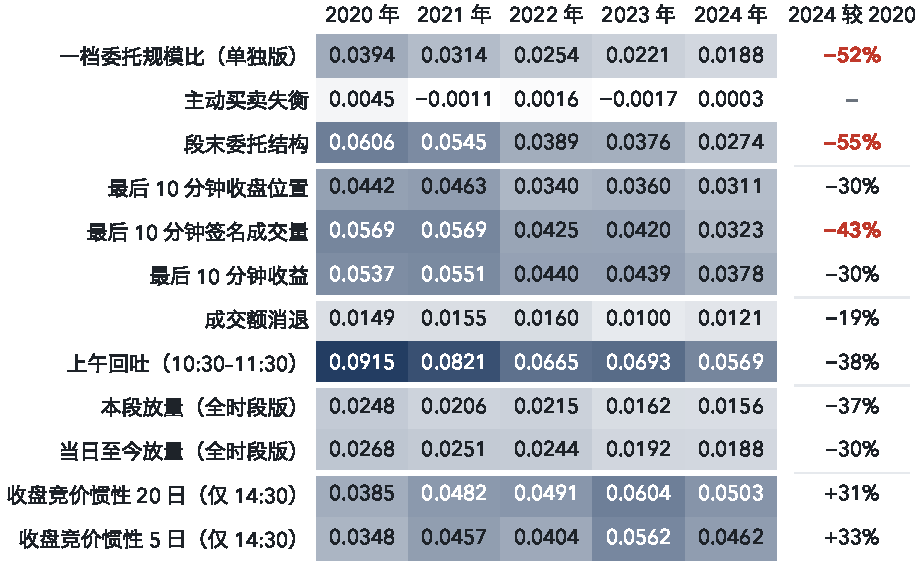
\includegraphics[width=\figwidth]{figures/fig_signal_decay_r.pdf}
\source{比赛平台分钟行情，团队本地评测}
\end{figure}

图表~\ref{fig:process} 按阶段列出研究过程：委托笔数单因子、多尺度反转、同伴残差与中性化、浅层树组合、16 个树平均、缓冲带与委托规模比、14:30 收盘竞价、缓冲前中性化、尾盘与关注度四项。上栏按各阶段首次提交公榜的日期排列；下栏是每日运行的本地评测任务数，三周内合计 6600 个，单日最多 937 个。

\begin{figure}[htbp]
\caption{研究分九个阶段推进，三周内运行 6600 个本地评测任务}\label{fig:process}
\centering
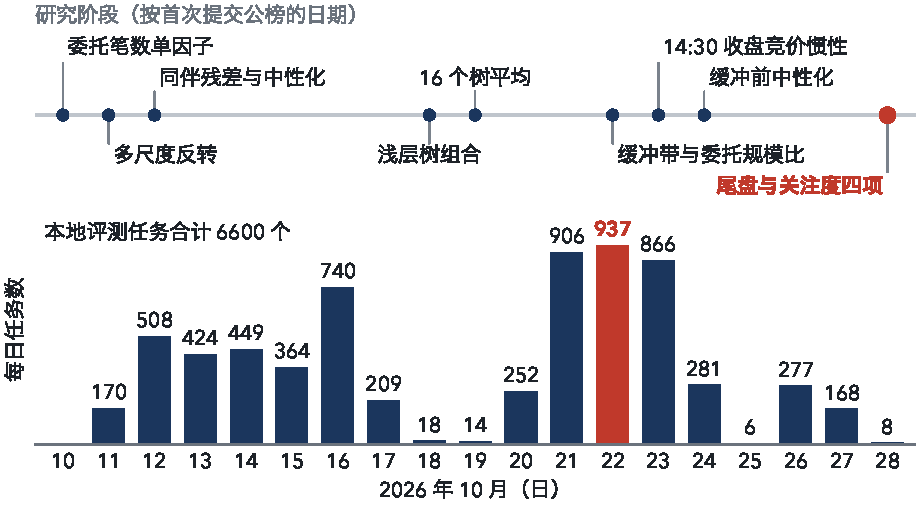
\includegraphics[width=\figwidth]{figures/fig_research_process_r.pdf}
\source{团队整理}
\end{figure}

图表~\ref{fig:milestones} 是各阶段代表版本的逐年 RankIC。每个版本的 RankIC 都在 2024 年最低：同伴残差反转（版本 C）2024 年为 0.0680，线性合成基准为 0.0713，基础组合为 0.0799，最终因子为 0.0842。浅层树相关版本的 2020–2022 年是拟合年份，没有列出。

\begin{figure}[htbp]
\caption{各阶段代表版本的 RankIC 都在 2024 年最低（本地评测）}\label{fig:milestones}
\centering
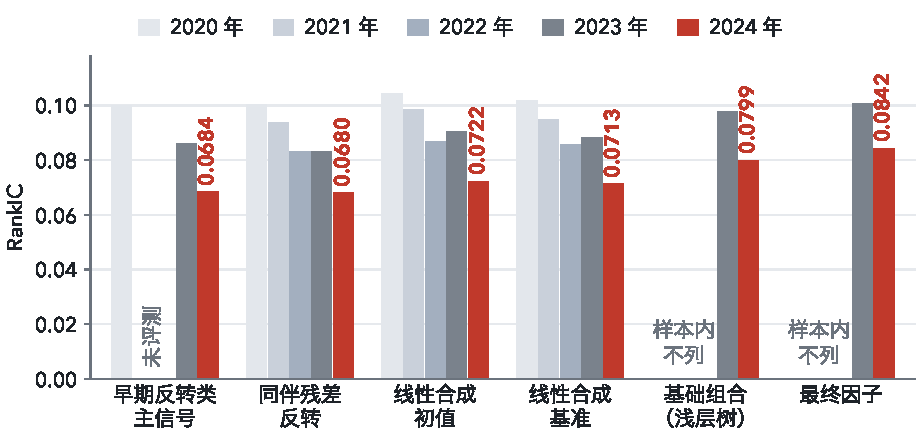
\includegraphics[width=0.72\figwidth]{figures/fig_milestones_by_year_r.pdf}
\source{比赛平台分钟行情，团队本地评测}
\end{figure}

\subsection*{H　术语表}\addcontentsline{toc}{subsection}{H　术语表}

\begin{table}[H]
\caption{本报告使用的术语（与正文首次出现时给出的定义一致）}\label{tab:terms}
\centering
{\tablesetup\renewcommand{\arraystretch}{1.0}
\begin{tabularx}{\textwidth}{@{}P{3.3cm} L@{}}
\toprule
术语 & 定义\\
\midrule
截面 & 每个交易日 8 个评测时点之一；截面 $t$ 只能使用 $t$ 及之前的数据\\
标签 & 截面之后 30 分钟窗口的收盘价除以同窗口成交量加权均价再减 1\\
风格与行业中性化 & 逐截面对 10 个风格因子与 32 个申万一级行业哑变量做含截距的最小二乘回归，取残差\\
多头组合、空头组合 & 每个截面残差排名前 10\%、后 10\% 的等权组合，合称多空名单\\
基础信号 & 输入基础组合的 27 个截面信号（附录 A）\\
基础组合 & 16 个浅层梯度提升树的平均，共 1920 棵树，只在 2020–2022 年拟合\\
增量信号 & 在基础组合输出上按小权重线性叠加的单项信号，共 15 项（附录 B）\\
同伴残差反转 & 相对走势最相似的一组股票的短期超涨超跌，再对规模、特质波动、非流动性、低价中性化\\
换手缓冲带 & 同一交易日内，上一截面已在名单内的股票划分名单时获得 $\beta$ 个标准差的保留优势；每天 10:00 重置\\
最小幅度调整 & 只把名单内低于“名单外最高者 $+\,m$”的股票调整到该值，其余保持原值\\
前一交易日暴露 & 中性化所用的风格暴露与行业取该股票上一条交易日记录\\
线性合成基准 & 同一批基础信号按线性权重合成的版本\\
本地评测系统 & 团队自建、与平台口径一致的评测程序，使用 2020–2024 年本地数据\\
准入标准 & RankIC、ICIR、多空组合夏普比率、压力稳定性四项不变差，换手率不升，至少一项明显更好，2023、2024 年分别判定\\
公榜同一页面比较 & 同一公榜页面上两个提交之间的比较；不同日期之间只比较五项原值\\
\bottomrule
\end{tabularx}}
\source{团队整理}
\end{table}

\subsection*{I　参考文献}\addcontentsline{toc}{subsection}{I　参考文献}

\begin{enumerate}[label={[\arabic*]},leftmargin=2.2em]
\item Da Z, Liu Q, Schaumburg E. A closer look at the short-term return reversal. Management Science, 2014.
\item Nagel S. Evaporating liquidity. Review of Financial Studies, 2012.
\end{enumerate}

\end{document}
